\documentclass{beamer}

\usetheme{focus} % Use the Focus theme supplied with the template
% Add option [numbering=none] to disable the footer progress bar
% Add option [numbering=fullbar] to show the footer progress bar as always full with a slide count
\usepackage{tikz}
\usepackage{amsmath}
\usepackage{amsfonts}
\usepackage{amssymb}
\usepackage{setspace}
\usepackage{algorithm2e}
\usepackage{algorithmic}
\newcommand{\predicate}[1]{\texttt{#1}}
\newcommand{\numberofgenes}[3][|T]{n_{#2#3#1}}
\newcommand{\numberofterms}[2][|T]{m_{#2#1}}
\newcommand{\ifgenehasactiveterm}{\text{if } \exists \; T_j \in T(H_i): T_j=1}
\newcommand{\gengo}{GenGO$^{\prime}$}
\newcommand{\btgK}{MGSA$^{\prime}$}  %%% B2G with KNOWN parameter values.
\newcommand{\btg}{MGSA}  %%% B2G with UNKNOWN parameter values
\newcommand{\argmax}{\operatornamewithlimits{arg\,max}}

\usepackage[most]{tcolorbox}
\usetikzlibrary{fadings,decorations.markings,arrows,shapes}
\tcbuselibrary{skins}
\newtcolorbox{mybluebox}[2][]{%
    colback=bg, 
    colframe=blue!75!black,
    fonttitle=\bfseries,
    coltitle=blue!75!black, 
    colbacktitle=bg,
    enhanced,
    attach boxed title to top left={yshift=-1.2mm, xshift=2mm},
  title=#2,
  #1}   


% Uncomment to enable the ice-blue theme
%\definecolor{main}{RGB}{92, 138, 168}
%\definecolor{background}{RGB}{240, 247, 255}

%------------------------------------------------

\usepackage{booktabs} % Required for better table rules

%----------------------------------------------------------------------------------------
%	 TITLE SLIDE
%----------------------------------------------------------------------------------------

\title{Overrepresetation: \\ Algorithms for Gene Ontology}

\subtitle{From Fisher to Bayes}

\author{Peter N Robinson}

\titlegraphic{
\includegraphics[scale=0.75]{img/JGMlogo.png}} % Optional title page image, comment this line to remove it

\institute{The Jackson Laboratory \\ Farmington CT}

\date{2022-10-18}

%------------------------------------------------

\begin{document}

%------------------------------------------------

\begin{frame}
	\maketitle % Automatically created using the information in the commands above
\end{frame}


\begin{frame}{Ontology Algorithms for Translational Research and Clinical Decision Support}
 \begin{mybluebox}{Game plan}
 Two lectures with assignments
 \end{mybluebox}
 
 \begin{itemize}
 \item My goal in these lectures is to provide insight into how to develop novel algorithms to address challenges in biomedical research and clinical decision support
 \item Understanding the domain, modelling the domain with ontologies (and schemas), writing algorithms to capture salient aspects of the data
 \item Today: Mainly Gene Ontology
 \item Next time: Mainly Human Phenotype Ontology
 \end{itemize}

\end{frame}



%----------------------------------------------------------------------------------------
%	 SECTION 1
%----------------------------------------------------------------------------------------

%\section{Gene Ontology} % Section title slide, unnumbered

%------------------------------------------------

%%%%%%%%%%%%%%%%%%%%%%%%%%%%%%%%%%%%%%%%%%%%%%%%%%%%%%%%%%%%%%%%%%%
%%%%%%%%%%%%%%%%%%%%%%%%%%%%%%%%%%%%%%%%%%%%%%%%%%%%%%%%%%%%%%%%%%%
\begin{frame}{Gene Ontology}
    \begin{mybluebox}{Gene Ontology (GO)}
    GO is being developed with the goal of providing a
    set of structured vocabularies for the annotation of genes and their products. Since    	the publication  of the original paper in \emph{Nature Genetics} in 2000, GO
    has become one of the most widely used and mature bio-ontologies,
    although it is still very much a work in progress~\cite{GO2019}.
    \end{mybluebox}
    
    \begin{figure}
     \centering
     
\includegraphics[width=0.25\textwidth]{./img/GOlogo.png}
    \end{figure}
    
\end{frame}

%------------------------------------------------

%%%%%%%
%%%%%%%%%%%%%%%%%%%%%%%%%%%%%%%%%%%%%%%%%%%%%%%%%%%%%%%%%%%%%%%%%%%%%%%%%%%%%%%%%%%%%%%%%%%%%%%%%%%%
\begin{frame}{Why do we need GO?}
\begin{itemize}
\item Exponential increase in biological data $\longmapsto$ need for databases with appropriate 
representation techniques
\item Progress in the way biologists describe functions has not kept pace with the results of 
large-scale sequencing projects $\longmapsto$ need for eff{}icient high-quality procedures for 
(preliminary) annotation of genes (e.g. \textit{Drosophila} genome)
\item Nomeclature for genes, gene products, and functions is widely divergent between dif{}ferent 
databases $\longmapsto$ too diff{}icult to compare between species

\item Uses: Information extraction, data mining, database integration...

\end{itemize}
\end{frame}

%%%%%%%%%%%%%%%%%%%%%%%%%%%%%%%%%%%%%%%%%%%%%%%
%%%%%%%%%%%%%%%%%%%%%%%%%%%%%%%%%%%%%%%%%%%%%%%

\begin{frame}{What came before GO?}
\begin{mybluebox}{Enzyme Commission}
    Before GO came on the scene, biological functions were represented as trees.
\end{mybluebox}
\vspace{-5mm}

\begin{center}
  \begin{tabular}{cp{5mm}c}
    \rotatebox{270}{ \resizebox{0.3\textheight}{!}{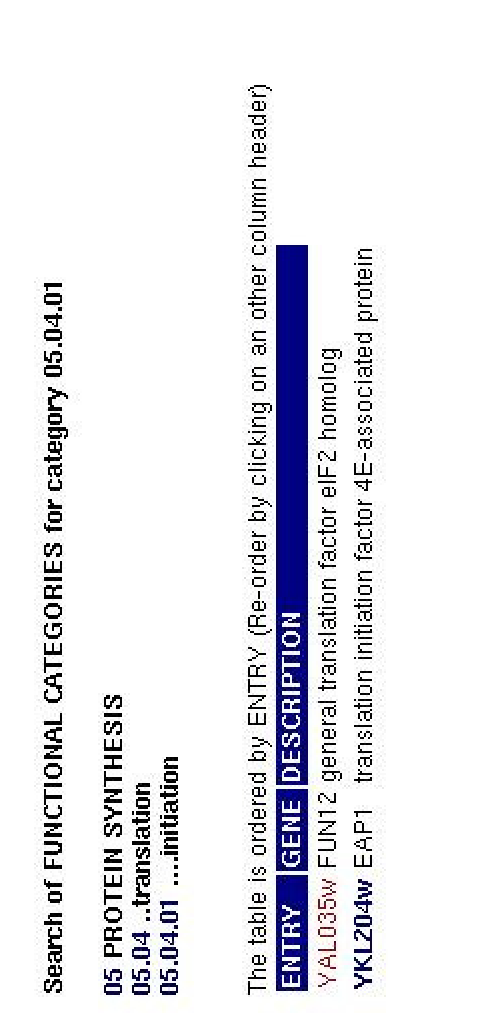
\includegraphics{img/mips.pdf}} }&
	&
     \rotatebox{270}{\resizebox{0.3\textheight}{!}{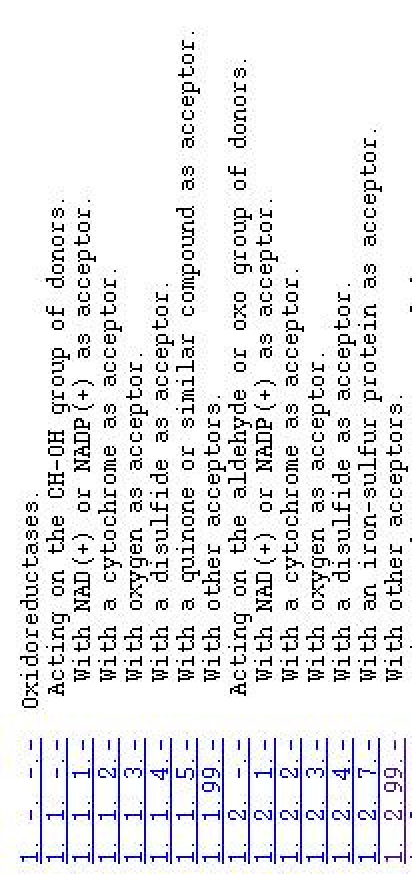
\includegraphics{img/EC.pdf}}} \\
 	MIPS & & EC \\
  \end{tabular}
\end{center}
\vspace{-2mm}
\begin{itemize}
\item MIPS: Munich Information Center for Protein Sequences
\item EC: Enzyme commision def{}initions of enzyme classes, subclasses and sub-subclasses
\end{itemize} 

\end{frame}

%%%%%%%%%%%%%%%%%%%%%%%%%%%%%%%%%%%%%%%%%%%%%%%
%%%%%%%%%%%%%%%%%%%%%%%%%%%%%%%%%%%%%%%%%%%%%%%

\begin{frame}{Function?}
The term function is sometimes used in a rather vague way..
\begin{itemize}
\item biochemical activity
\item biological goals
\item subcellular localization
\end{itemize} 

\begin{figure}
\centering
\rotatebox{270}{
\resizebox{0.5\textheight}{!}{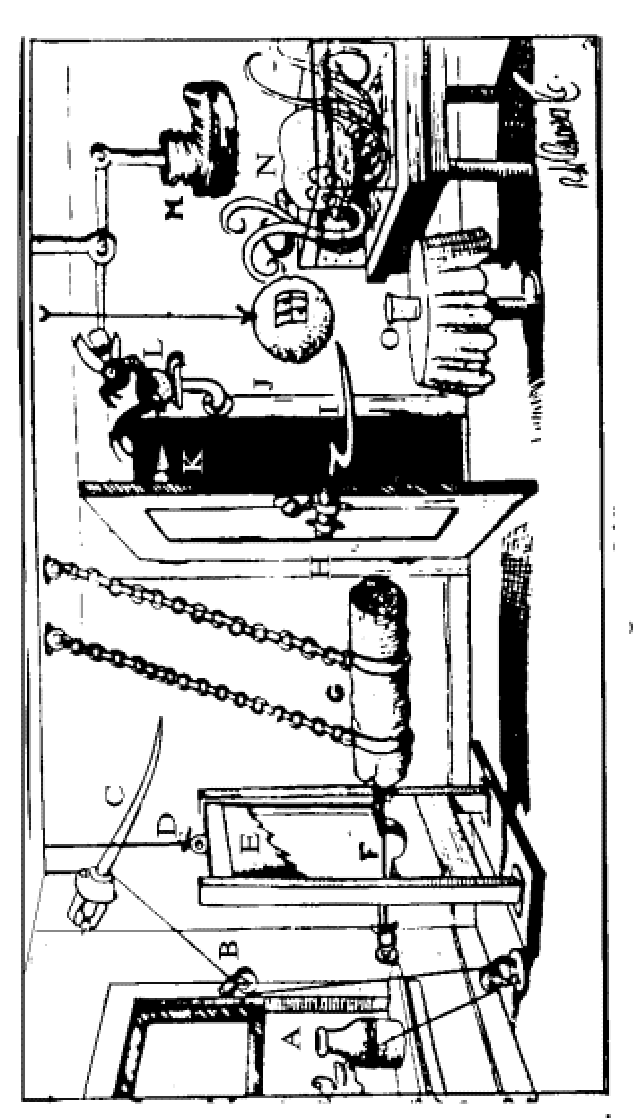
\includegraphics{img/rube.pdf}}
}
\end{figure}

\end{frame}


%%%%%%%%%%%%%%%%%%%%%%%%%%%%%%%%%%%%%%%%%%%%%%%
%%%%%%%%%%%%%%%%%%%%%%%%%%%%%%%%%%%%%%%%%%%%%%%

\begin{frame}{GO: Biological Process}
\begin{itemize}
\item Biological objective to which the gene or gene product contributes
\item A process is accomplished by one or more assemblies of molecular functions
\item Often involve chemical or physical transformation
\item Examples: (High level) \textquotedblleft Signal Transduction\textquotedblright, 
\textquotedblleft Cell Growth and Maintenance\textquotedblright
\item Examples: (Lower level) \textquotedblleft pyrimidine metabolism\textquotedblright, 
\textquotedblleft cAMP biosynthesis\textquotedblright
\end{itemize}
\end{frame}

%%%%%%%%%%%%%%%%%%%%%%%%%%%%%%%%%%%%%%%%%%%%%%%
%%%%%%%%%%%%%%%%%%%%%%%%%%%%%%%%%%%%%%%%%%%%%%%

\begin{frame}{GO: Biological Process (2)}
\begin{center}
\rotatebox{270}{
\resizebox*{!}{1\textheight}{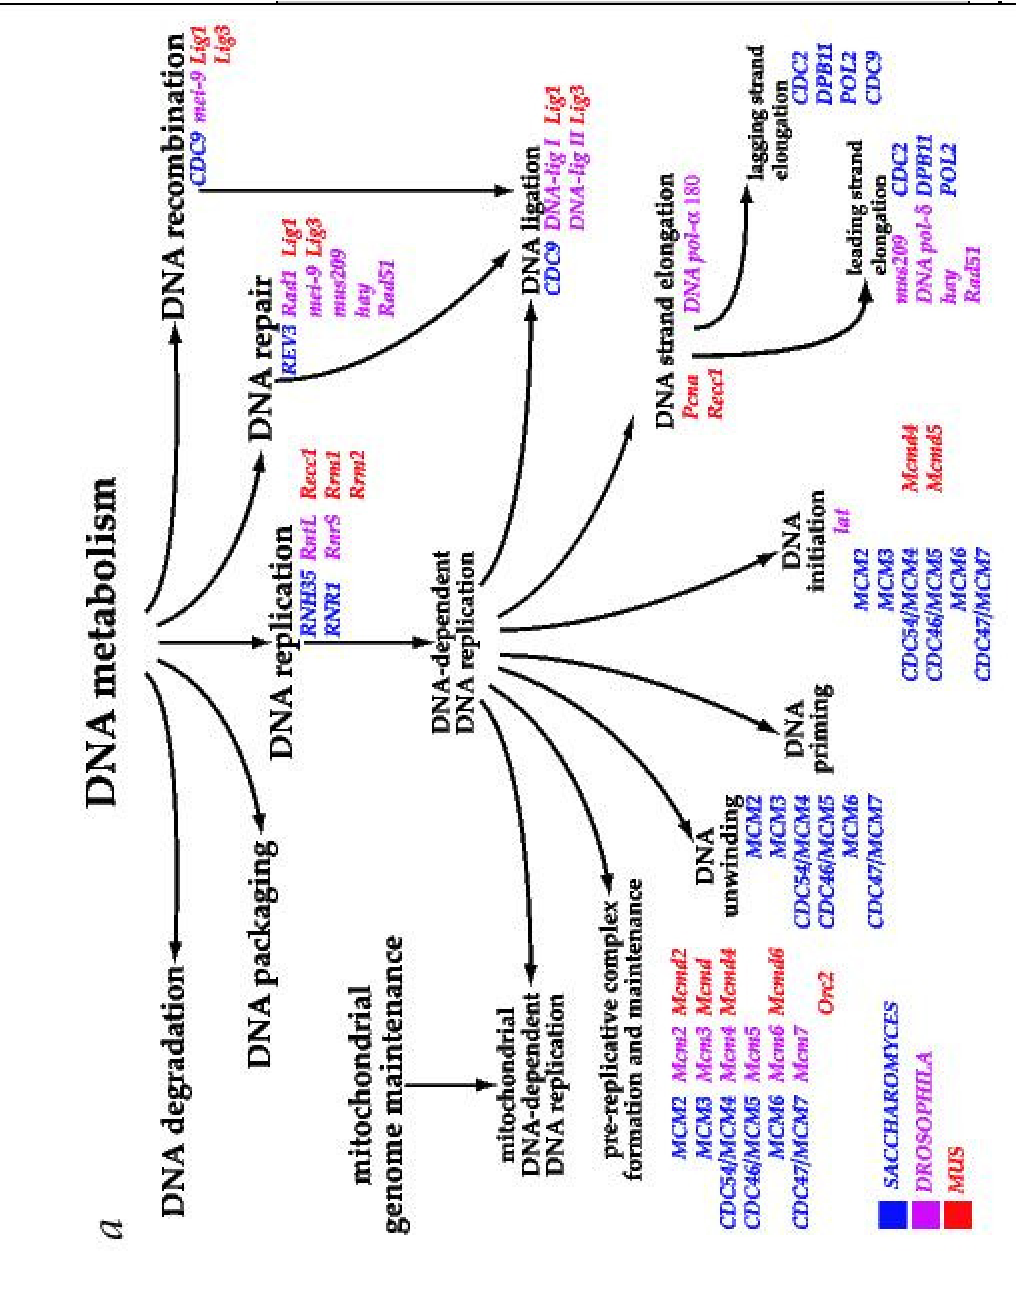
\includegraphics{img/dnametabolism.pdf}}
}
\end{center}
\end{frame}

%%%%%%%%%%%%%%%%%%%%%%%%%%%%%%%%%%%%%%%%%%%%%%%
%%%%%%%%%%%%%%%%%%%%%%%%%%%%%%%%%%%%%%%%%%%%%%%

\begin{frame}{GO: Molecular Function}
\begin{itemize}
\item Biochemical activity of a gene product
\item describes \textit{what} is done rather than why or where or when
\item Examples: (High level) \textquotedblleft Enzyme',  \textquotedblleft 
transporter\textquotedblright
\item Examples: (Lower level) \textquotedblleft adenylate cyclase\textquotedblright, 
\textquotedblleft Toll receptor ligand\textquotedblright
\end{itemize}
\end{frame}
%%%%%%%%%%%%%%%%%%%%%%%%%%%%%%%%%%%%%%%%%%%%%%%
%%%%%%%%%%%%%%%%%%%%%%%%%%%%%%%%%%%%%%%%%%%%%%%
\begin{frame}{GO: Molecular Function (2)}
\begin{center}
\rotatebox{270}{
\resizebox*{!}{1\textheight}{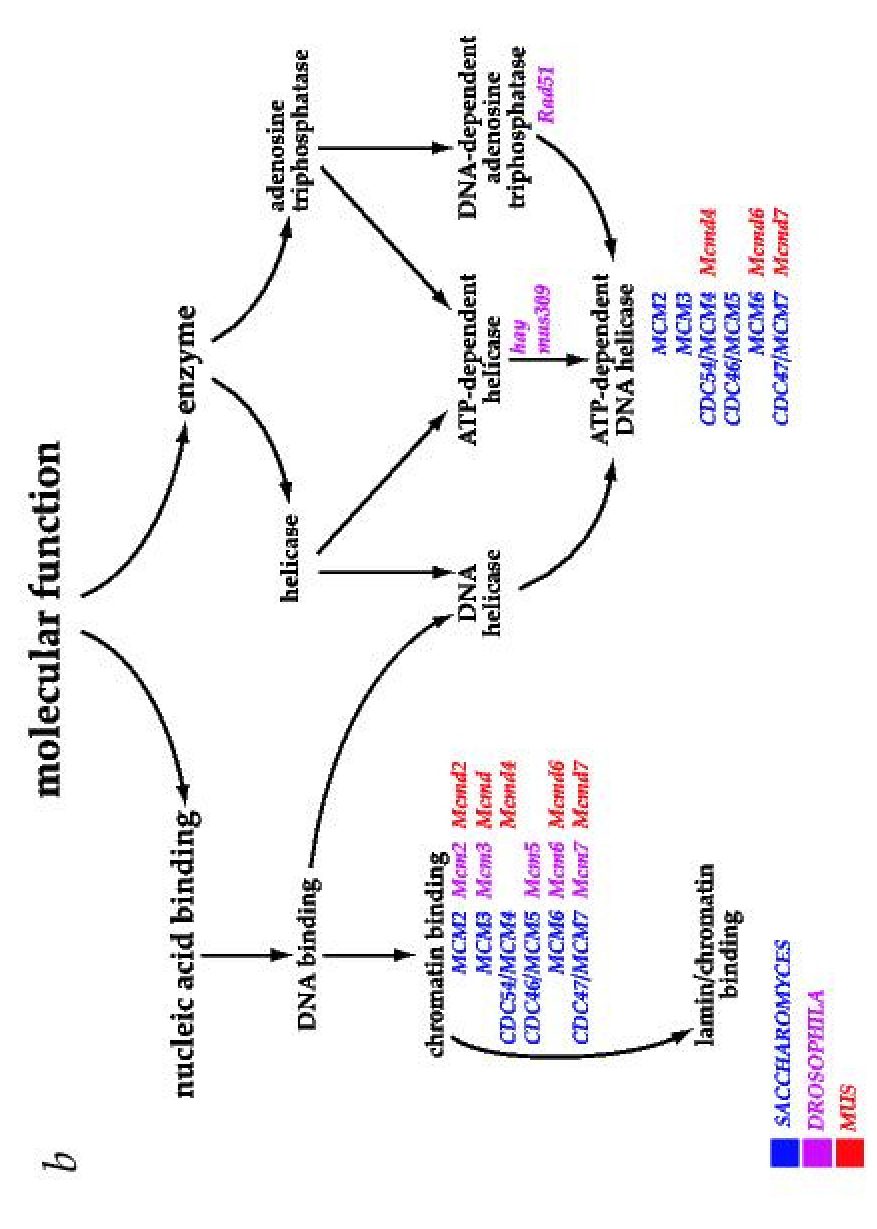
\includegraphics{img/molecularfun.pdf}}
}
\end{center}
\end{frame}

%%%%%%%%%%%%%%%%%%%%%%%%%%%%%%%%%%%%%%%%%%%%%%%
%%%%%%%%%%%%%%%%%%%%%%%%%%%%%%%%%%%%%%%%%%%%%%%
\begin{frame}{GO: Cellular component}
\begin{itemize}
\item Place in the cell where a gene product is active
\item Example: \textquotedblleft Nuclear membrane\textquotedblright
\item Can also refer to entities made up of multiple gene products are to be found
\item Example: \textquotedblleft ribosome\textquotedblright, \textquotedblleft 
proteosome\textquotedblright
\end{itemize}
\end{frame}
%%%%%%%%%%%%%%%%%%%%%%%%%%%%%%%%%%%%%%%%%%%%%%%
%%%%%%%%%%%%%%%%%%%%%%%%%%%%%%%%%%%%%%%%%%%%%%%
\begin{frame}{GO: Cellular component (2)}
\begin{center}
\rotatebox{270}{
\resizebox*{!}{1\textheight}{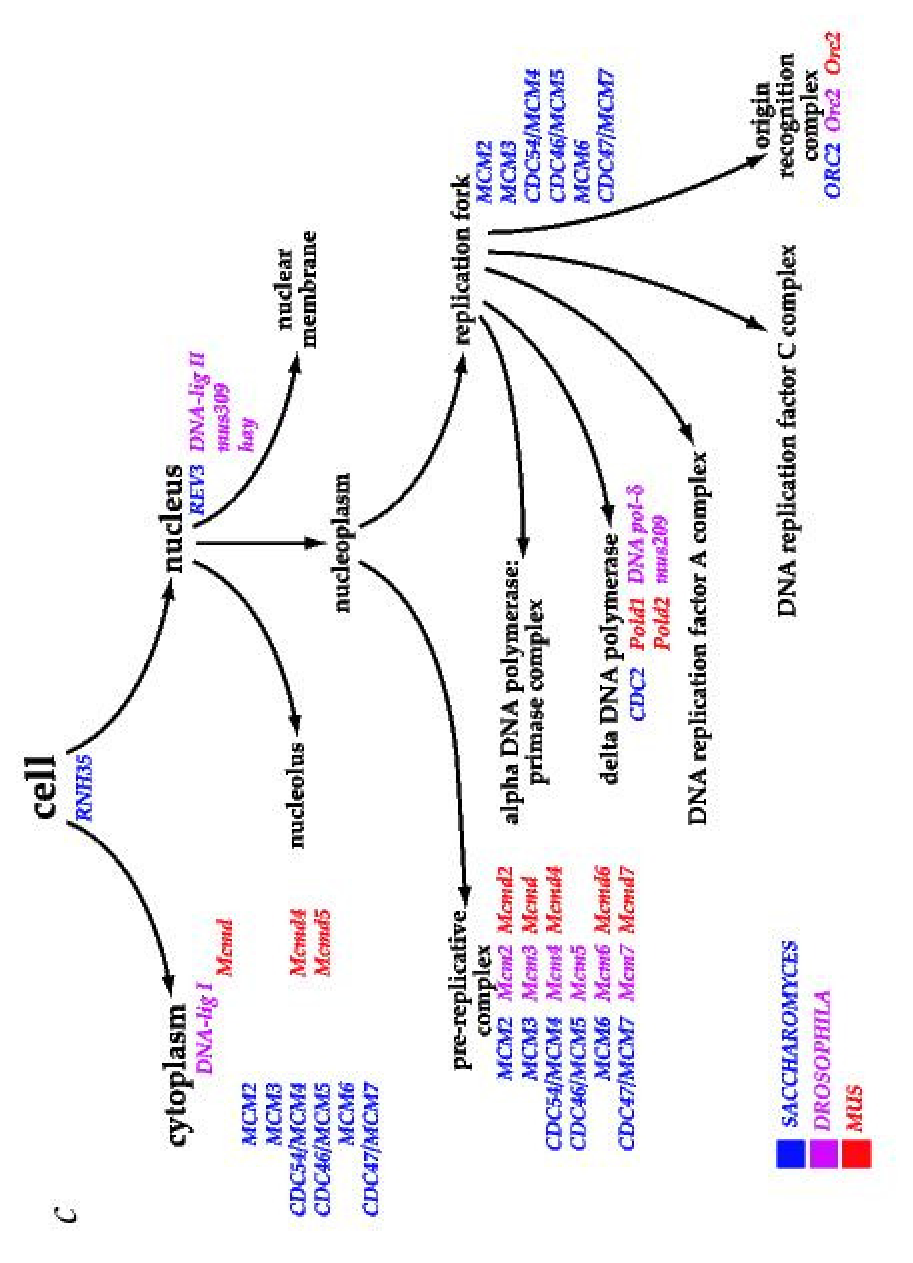
\includegraphics{img/cellcomponent.pdf}}
}
\end{center}
\end{frame}
%%%%%%%%%%%%%%%%%%%%%%%%%%%%%%%%%%%%%%%%%%%%%%%
%%%%%%%%%%%%%%%%%%%%%%%%%%%%%%%%%%%%%%%%%%%%%%%

% GO terms
\begin{frame}{GO Terms}
\begin{itemize}
\item GO:0003678
\item Name: DNA helicase activity
\item Def{}inition: Catalysis of the the hydrolysis of ATP to unwind the DNA helix at the 
replication fork, allowing the resulting single strands to be copied.
\item Information about parent terms (bookkeeping of the DAG structure)
\end{itemize} 
\begin{small}Each entry (\textit{term}) in GO contains this information\end{small}
\end{frame}
%%%%%%%%%%%%%%%%%%%%%%%%%%%%%%%%%%%%%%%%%%%%%%%
%%%%%%%%%%%%%%%%%%%%%%%%%%%%%%%%%%%%%%%%%%%%%%%


\begin{frame}{GO Annotations}
\begin{itemize}
\item Annotations are available for numerous species
\item GO can be regarded as an {\bf attribute ontology}
\end{itemize}
\begin{center}
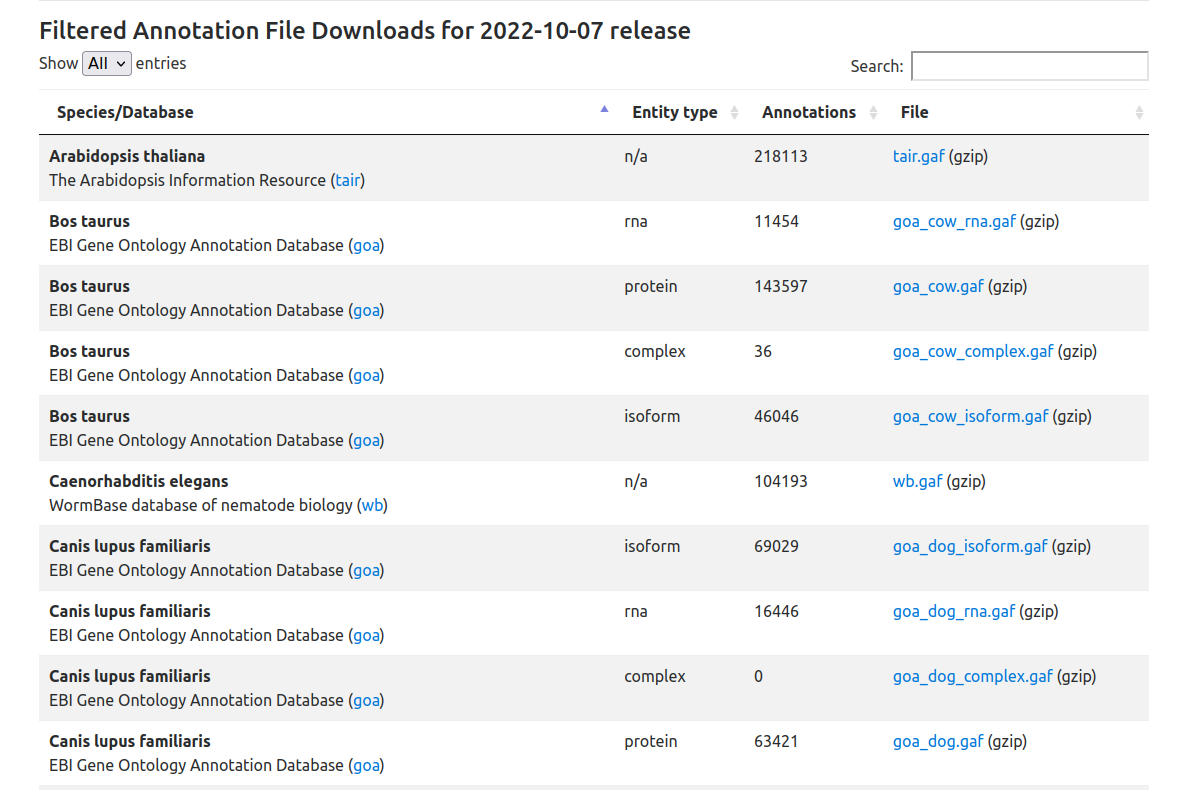
\includegraphics[width=0.7\textwidth]{img/go-gaf-page.png}
\end{center}
\begin{flushleft}
\begin{tiny}\textit{http://current.geneontology.org/products/pages/downloads.html}\end{tiny}
\end{flushleft}
\end{frame}

%%%%%%%%%%%%%%%%%%%%%%%%%%%%%%%%%%%%%%%%%%%%%%%
%%%%%%%%%%%%%%%%%%%%%%%%%%%%%%%%%%%%%%%%%%%%%%%

\begin{frame}{Example: fibrillin-1}
\begin{itemize}
\item Annotations are made for biological process, molecular function, and cellular component
\item evidence and source of the assertion (not shown)
\end{itemize} 

\begin{center}
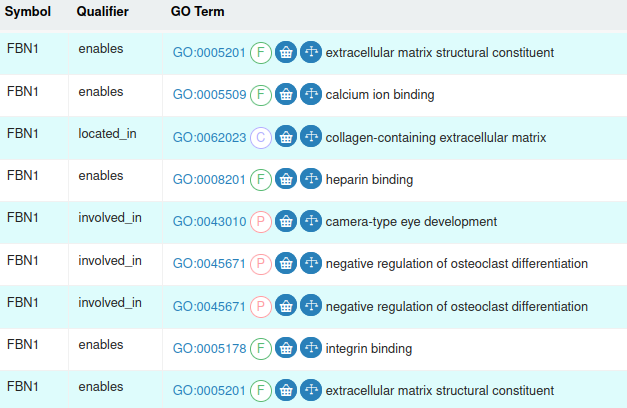
\includegraphics[width=0.7\textwidth]{img/fbn1-goa.png}
\end{center}
\end{frame}


%%%%%%%%%%%%%%%%%%%%%%%%%%%%%%%%%%%%%%%%%%%%%%%
%%%%%%%%%%%%%%%%%%%%%%%%%%%%%%%%%%%%%%%%%%%%%%%
\begin{frame}{GO: Overrepresentation Analysis}
\begin{mybluebox}{Question}
We have done a high throughput experiment and identified a list of differentially 
expressed genes. What are the salient characteristics of the genes in this list?
\end{mybluebox}

 \begin{itemize}
  \item We could just count the number of genes annotated to a certain GO term, but commomn things are common
  \item Instead, GO analysis asks the question of whether a given GO term is annotated {\bf more often than we would expect by chance}
\item Today, we will explain some algorithms for addressing this question. Similar approaches can be taken with other ontologies in a range of biological and medical settings.
 \end{itemize}

\end{frame}



%%%%%%%%%%%%%%%%%%%%%%%%%%%%%%%%%%%%%%%%%%%%%%%
%%%%%%%%%%%%%%%%%%%%%%%%%%%%%%%%%%%%%%%%%%%%%%%
\begin{frame}{binomial coefficient}
\begin{mybluebox}{Question?}
How do we calculate how many different sequences of outcomes there are if we flip a coin $n$ times?
\end{mybluebox}
\begin{columns}
\column{0.7\textwidth}
\begin{itemize}
\item  Each of the $n!$ rearrangements of the
numbers $1,2,\ldots,n$ defines a different rearrangement of the
letters $HHH\ldots HHTT\ldots TT$.
\item However, not all of the
rearrangements change the order of the $H$'s and the $T$'s. For
instance, exchanging the first two positions leaves the order
$HHH\ldots HHTT\ldots TT$ unchanged.
\end{itemize}
\column{0.3\textwidth}

\begin{center}
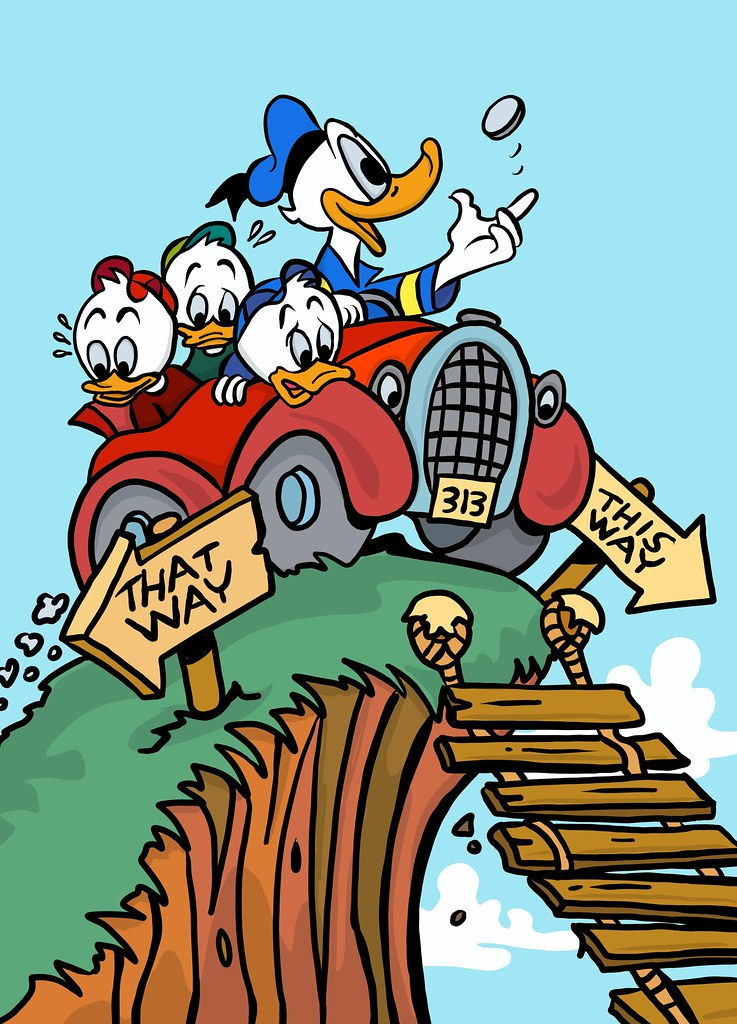
\includegraphics[width=1\textwidth]{img/donald.png}
\end{center}
\end{columns}

\end{frame}


%%%%%%%%%%%%%%%%%%%%%%%%%%%%%%%%%%%%%%%%%%%%%%%
%%%%%%%%%%%%%%%%%%%%%%%%%%%%%%%%%%%%%%%%%%%%%%%
\begin{frame}{binomial coefficient}

 \begin{mybluebox}{``$n$ choose $k$''}
The quantity $ \binom{n}{k} $ (read ``$n$ choose $k$'') is known as the binomial
coefficient.
\end{mybluebox}

 
\begin{itemize}
\item How do we calculate how many different sequences of outcomes there are if we flip a coin $n$ times?
\end{itemize}

  Noting that there are $k!$ ways of reordering the
``heads'' and $(n-k)!$ ways of reordering the ``tails,'' it follows
that there are
\begin{equation}
 \binom{n}{k} = \dfrac{n!}{\left(n-k\right)! k!}
\label{eq:binomial-coefficient}
\end{equation}
different ways of rearranging $k$ ``heads'' and $n-k$ ``tails.'' 

 
\end{frame}
%%%%%%%%%%%%%%%%%%%%%%%%%%%%%%%%%%%%%%%%%%%%%%%
%%%%%%%%%%%%%%%%%%%%%%%%%%%%%%%%%%%%%%%%%%%%%%%
\begin{frame}{binomial coefficient}
 \begin{mybluebox}{$k$ successes in $n$ attempts}
We are interested in the probability
of any one particular order of trials with $k$ successes and $n-k$
failures, we multiply the probabilities of the individual trials to
obtain $p^k(1-p)^{n-k}$. 
\end{mybluebox}

\begin{itemize}
\item We simply multiply the probability of one
particular trial order with $k$ successes and $n-k$ failures  by the number of trial
orders resulting in $k$ successes. 
\item This probability distribution is called the
\index{binomial distribution}
\textit{binomial distribution}:
\end{itemize}



\begin{equation}
 \label{eq:dbinomial}
P(k,n,p) = \binom{n}{k} p^k\left(1-p\right)^{n-k}
\end{equation} 
 
\end{frame}
%%%%%%%%%%%%%%%%%%%%%%%%%%%%%%%%%%%%%%%%%%%%%%%
%%%%%%%%%%%%%%%%%%%%%%%%%%%%%%%%%%%%%%%%%%%%%%%
\begin{frame}{binomial coefficient}


\begin{figure}[h!]
 \centering
 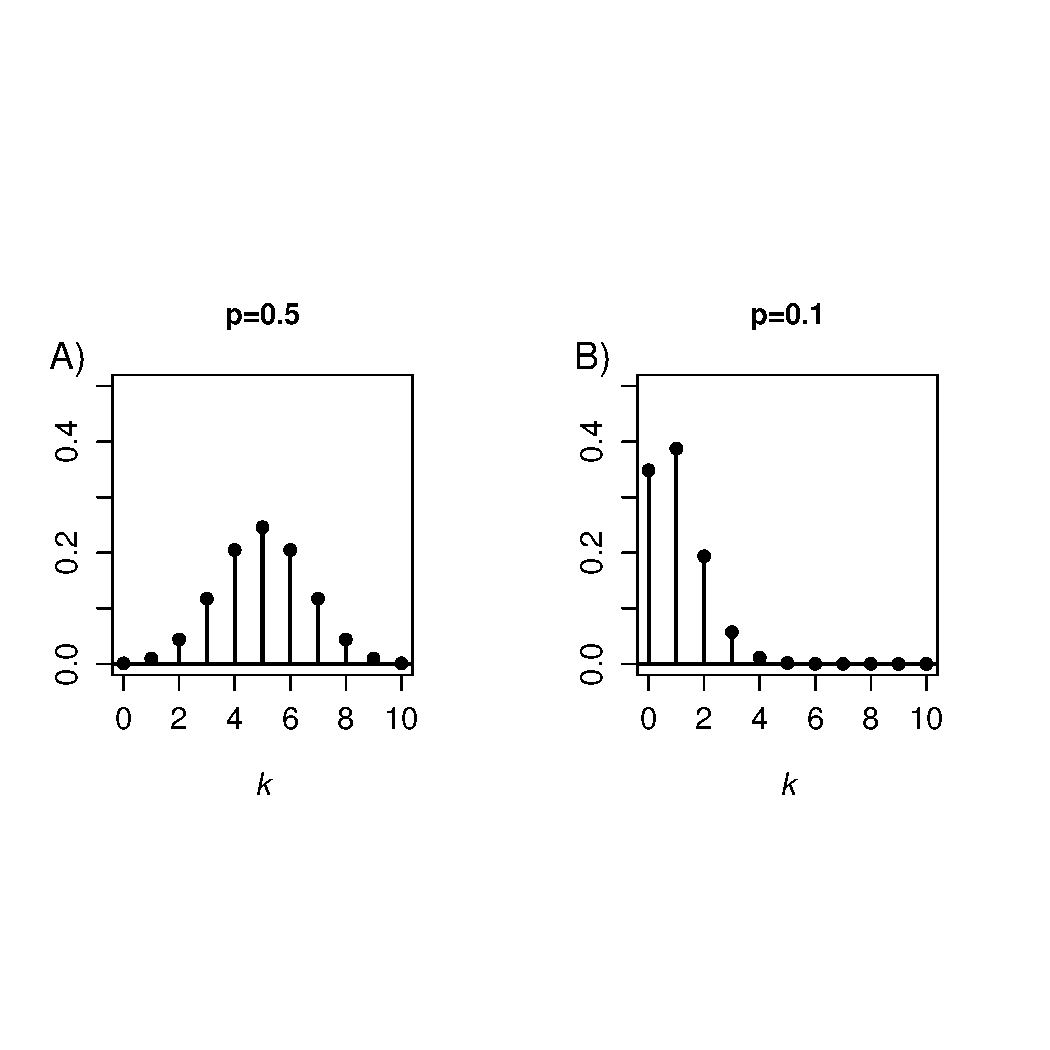
\includegraphics[width=.8\textwidth,viewport= 0 100 500 
380,clip]{img/binomial.pdf}
 \label{fig:binomial}
\end{figure}
\begin{description}
\item[A]the probability of
   $k=1,\ldots,10$ ``heads'' in ten coin tosses using a fair coin
   ($p=0.5$). 
   \item[B]Probability of $k=1,\ldots,10$ ``heads''
   in ten coin tosses using a biased coin ($p=0.1$).
\end{description} 
 
 

\end{frame}
%%%%%%%%%%%%%%%%%%%%%%%%%%%%%%%%%%%%%%%%%%%%%%%
%%%%%%%%%%%%%%%%%%%%%%%%%%%%%%%%%%%%%%%%%%%%%%%
\begin{frame}{GO Overrepresentation with the binomial distribution}
 \begin{mybluebox}{GO overrepresentation analysis}
each gene in the study set
is considered to be a ``trial,''  and ``success'' occurs if the gene is
annotated to a GO term of interest.
\end{mybluebox}
\begin{itemize}
\item The probability of ``success'' is simply the
frequency of the annotation to the GO term among all genes.  For
instance, if there are 10,000 genes are sequenced in an RNA-seq experiment, 600 of which
are annotated to some GO term $t$, then the probability of $t$ is
 $p=\frac{600}{10,000}=0.06$
\item If there are 250 differentially expressed genes, 30 of which are annotated to $t$, we can approximate the probability of observing exactly 30 genes in
the DE set annotated to $t$ as
\end{itemize}
\begin{equation}
\mathrm{P}(30,250,0.06)=1.44\times 10^{-4}
\end{equation}

 
\end{frame}
%%%%%%%%%%%%%%%%%%%%%%%%%%%%%%%%%%%%%%%%%%%%%%%
%%%%%%%%%%%%%%%%%%%%%%%%%%%%%%%%%%%%%%%%%%%%%%%
\begin{frame}{GO Overrepresentation}
 \begin{mybluebox}{null hypothesis}
 In order to use this for a statistical test,
 we now define a \textit{null hypothesis} to be
that the biological function described by GO term $t$ is not
overrepresented among the differentially expressed genes
\end{mybluebox}


\begin{itemize}
 \item if we
symbolize the proportion of genes in the population and study set that
are annotated to the term as $\pi_p$ and $\pi_s$, then
\end{itemize}
\begin{equation}
H_0:\pi_{s}\leq\pi_p 
\end{equation}

\end{frame}


%%%%%%%%%%%%%%%%%%%%%%%%%%%%%%%%%%%%%%%%%%%%%%%
%%%%%%%%%%%%%%%%%%%%%%%%%%%%%%%%%%%%%%%%%%%%%%%
\begin{frame}{GO Overrepresentation}
\begin{mybluebox}{alternative hypothesis}
Some GO term $t$ annotates a higher than expected proportion of the genes
in the study set.
\end{mybluebox}

\begin{equation}
H_A:\pi_{s}>\pi_p 
\end{equation}

\begin{itemize}
\item If the probability of the observed result of our experiment
(the observation of 30 genes in the DE set being annotated to $t$) is
less than $\alpha$, we reject the null hypothesis in favor of the
alternative hypothesis
\item This  would imply that the GO term $t$ has
something to do with the observed differential expression.
\end{itemize}


\end{frame}

%%%%%%%%%%%%%%%%%%%%%%%%%%%%%%%%%%%%%%%%%%%%%%%
%%%%%%%%%%%%%%%%%%%%%%%%%%%%%%%%%%%%%%%%%%%%%%%
\begin{frame}{GO Overrepresentation }
\begin{mybluebox}{Upper tail}
We calculate the probability of $\pi_{s}>\pi_p $ by calculating the probability of observing $k^{'}$ DE genes annotated to $t$ {\bf or more}, up to the maximum number of genes annotated to $t$ (because of only 100 gene are annotated to $t$, the probabilty of observing 101 or more is zero)
\end{mybluebox}

\begin{itemize}
\item  We take the sum to the maximum of the
number of genes annotated to a GO term $t$ (denoted $p_t$) or to the
size of the DE set (denoted $|\textit{DE}|$). 
\end{itemize}



\begin{equation}
 \label{eq:tailsumdbinomial}
p(k \geq k^{'},n,p) = \sum_{k=k^{'}}^{\min(p_t,|\textit{DE}|)}\binom{n}{k} 
k^p\left(n-k\right)^{1-p}.
\end{equation}  
 
 
\end{frame}

%%%%%%%%%%%%%%%%%%%%%%%%%%%%%%%%%%%%%%%%%%%%%%%
%%%%%%%%%%%%%%%%%%%%%%%%%%%%%%%%%%%%%%%%%%%%%%%
\begin{frame}{binomial distribution: Example}
 \begin{figure}[h!]
 \centering
 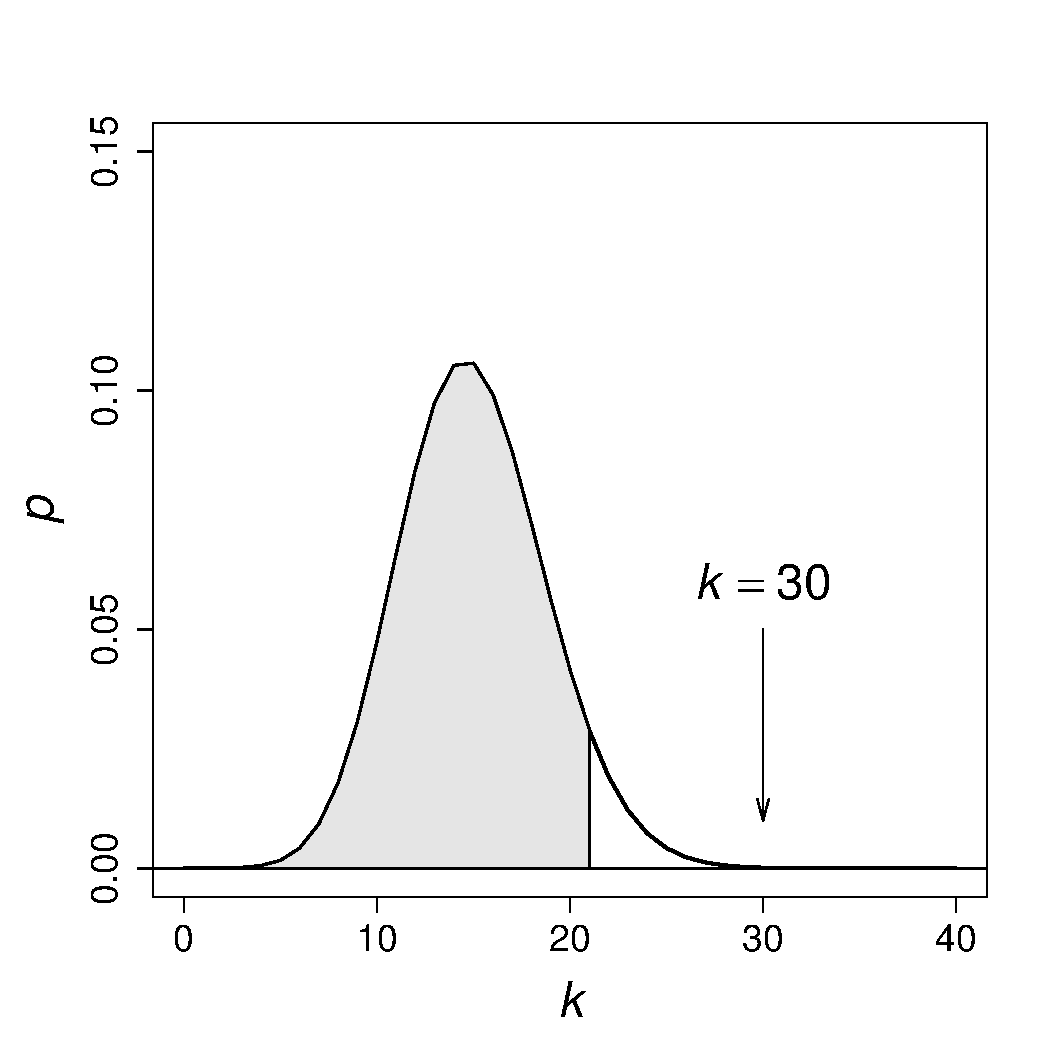
\includegraphics[width=0.4\textwidth]{img/Gobinom.pdf}
\end{figure}
\begin{scriptsize}Probability mass function (PMF)  with $p=0.06$ and
   $n=250$. Values for $k=0,1,\ldots,40$ are shown (the values for
   $k>40$ are nearly zero and are not shown). The observed value for
   $k$ of 30 lies outside of the range containing 95\% of the
   probability mass, and we reject the null hypothesis that the genes
   in the study set are not enriched in genes annotated by $t$. The
   $p$-value for this observation can be calculated by
   Equation~(\ref{eq:dbinomial}) to be $1.68\times 10^{-8}$.\end{scriptsize}
 
\end{frame}

%%%%%%%%%%%%%%%%%%%%%%%%%%%%%%%%%%%%%%%%%%%%%%%
%%%%%%%%%%%%%%%%%%%%%%%%%%%%%%%%%%%%%%%%%%%%%%%
\begin{frame}{To replace or not to replace}
\begin{mybluebox}{To replace or not to replace}
The individual tests are not independent if we do not replace drawn balls
\end{mybluebox}
\begin{figure}
\centering
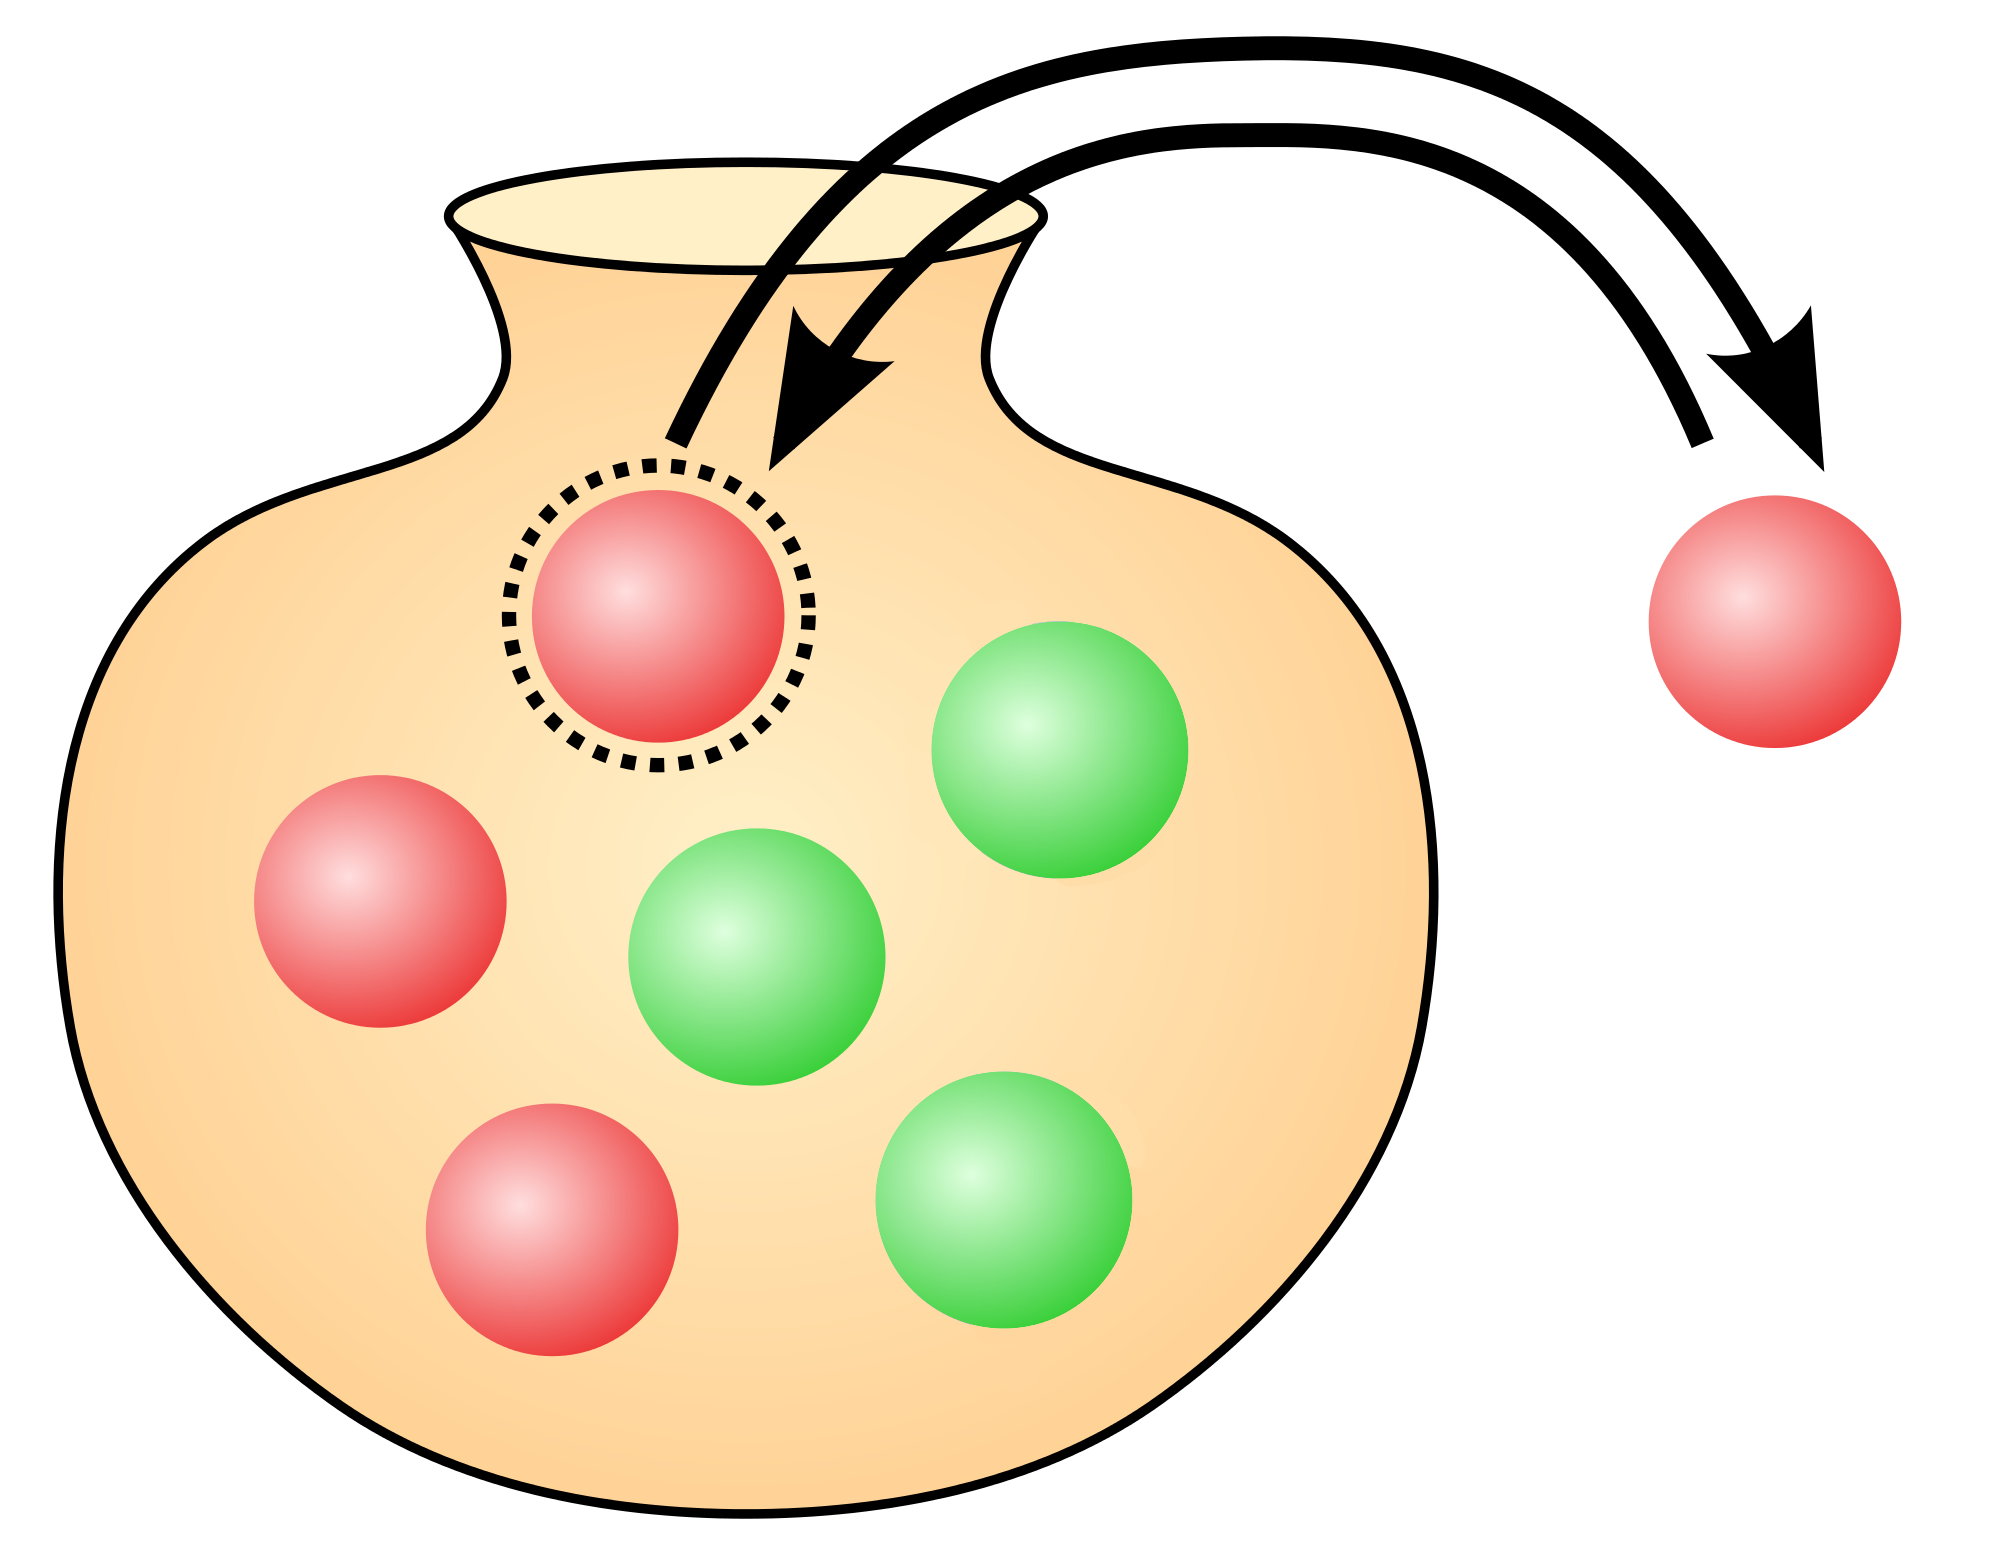
\includegraphics[width=0.4\textwidth]{img/urn.png} 

\end{figure}
\begin{itemize}
\item What is the probability of drawing a green ball if we replace the drawn red ball?
\item What is the probability  if we do not replace?

\end{itemize}

\end{frame}




%%%%%%%%%%%%%%%%%%%%%%%%%%%%%%%%%%%%%%%%%%%%%%%
%%%%%%%%%%%%%%%%%%%%%%%%%%%%%%%%%%%%%%%%%%%%%%%
\begin{frame}{binomial vs hypergeometric distribution}
\begin{mybluebox}{Faulty assumption}
 Although this approach provides a nearly correct answer for terms with
many annotations in the population and large DE sets, it is actually
only an approximation. 
\end{mybluebox}
\begin{itemize}
\item The problem is that the binomial distribution
is based on the assumption that the individual trials are independent
of one another. 
\item While this is clearly true for coin tosses, it is not
for GO overrepresentation analysis, which is rather comparable to a
lotto game in which labelled balls are taken from an urn and not
replaced.
\end{itemize}


\end{frame}



%%%%%%%%%%%%%%%%%%%%%%%%%%%%%%%%%%%%%%%%%%%%%%%
%%%%%%%%%%%%%%%%%%%%%%%%%%%%%%%%%%%%%%%%%%%%%%%

\begin{frame}{GO Overrepresentation with the hypergeometric distribution}
\begin{itemize}
\item In our
RNA-seq experiment, we imagine that the set of all 10,000 genes is represented by an urn with 10,000 balls.
\item  A total of 100 genes are
annotated to some GO term $t$, and thus 100 balls in the urn are
colored blue.
\item We then model the observation of 250 differentially
expressed genes as the process of randomly removing 250 balls in turn
from the urn {\bf without replacement}. 
\end{itemize}
   
\end{frame}


%%%%%%%%%%%%%%%%%%%%%%%%%%%%%%%%%%%%%%%%%%%%%%%
%%%%%%%%%%%%%%%%%%%%%%%%%%%%%%%%%%%%%%%%%%%%%%%
\begin{frame}{Hypergeometric distribution}
\begin{mybluebox}{Approach}
count up all the ways of getting $k$ genes annotated to $t$ and $n-k$
remaining genes not annotated to $t$, and compare this number to the
number of all possible outcomes. 
\end{mybluebox}

\begin{tabular}{ll}
$m$ & total number of genes\\
$m_t$ & number of those genes that are annotated to GO term $t$\\
$n$ & number of DE genes (study set) \\
$k$& the number of DE genes that are annotated to $t$\\
\end{tabular}

\vspace{4mm}

\begin{equation}
 \label{eq:hypergeometric}
p(k,n,p)  = \dfrac{\binom{m_t}{k}\binom{m-m_t}{n-k}}{\binom{m}{n}}.
\end{equation}
\end{frame}



%%%%%%%%%%%%%%%%%%%%%%%%%%%%%%%%%%%%%%%%%%%%%%%
%%%%%%%%%%%%%%%%%%%%%%%%%%%%%%%%%%%%%%%%%%%%%%%
\begin{frame}{GO Overrepresentation with the hypergeometric distribution}
\begin{mybluebox}{Probability of exactly $m_t$ annotated genes in study set}
 \begin{equation}
p(k,n,p)  = \dfrac{\binom{m_t}{k}\binom{m-m_t}{n-k}}{\binom{m}{n}}.
\end{equation}
\end{mybluebox}

\begin{itemize}
 \item There are $\binom{m_t}{k}$ ways of
choosing $k$ genes annotated to $t$.
\item There are $\binom{m-m_t}{n-k}$
ways of choosing the remaining $n-k$ genes that are not annotated to
$t$.
\item   In total, there are $\binom{m_t}{k}\binom{m-m_t}{n-k}$ ways of
choosing the genes in the study set such that $k$ are annotated to $t$
and $n-k$ are not. 
\item There are $\binom{m}{n}$ total ways of choosing a
study set with $n$ genes from the population of $m$ genes with
arbitrary annotations.
\end{itemize}


 
\end{frame}

%%%%%%%%%%%%%%%%%%%%%%%%%%%%%%%%%%%%%%%%%%%%%%%
%%%%%%%%%%%%%%%%%%%%%%%%%%%%%%%%%%%%%%%%%%%%%%%
\begin{frame}{Fisher's exact test}
\begin{mybluebox}{Probability of at least $m_t$ annotated genes in study set}
Equation~(\ref{eq:hypergeometric}) is known as the \textit{hypergeometric
distribution}. Analogously to the situation with the binomial
distribution, we need to calculate the probability of observing  $k^{'}$ {\bf or more} genes annotated to $t$ in order to have a
statistical test. 
\end{mybluebox}
 \begin{itemize}
 \item The sum over the tail of the
hypergeometric distribution is known as the \textbf{Exact Fisher
  Test}:
 \end{itemize}

\index{exact Fisher test}
\begin{equation}
 \label{eq:exactFisher}
p(K\geq k^{'},n,p) = 
\sum_{k=k^{'}}^{\min(K,|DE|)}\dfrac{\binom{m_t}{k}\binom{m-m_t}{n-k}}{\binom{m}{n}}
\end{equation}
 
 
\end{frame}

%%%%%%%%%%%%%%%%%%%%%%%%%%%%%%%%%%%%%%%%%%%%%%%
%%%%%%%%%%%%%%%%%%%%%%%%%%%%%%%%%%%%%%%%%%%%%%%
\begin{frame}{Term-for-Term}
 The standard approach to identify the most interesting terms is to
perform Fisher's exact test for each term separately. For this reason,
we refer to this procedure as the term-for-term (TfT)
approach

\begin{itemize}
 \item For each GO term $t$, the genes in the population set $M$ are either
annotated to term $t$ or not.
\item This divides the population set into two
classes of items, comparable to an urn with white and
black marbles. 
\item We denote the set of all genes in the population that
are annotated to GO term $t$ as  $M_t$ and the cardinality of the set
as $m_t$.
\end{itemize}

 
\end{frame}
%%%%%%%%%%%%%%%%%%%%%%%%%%%%%%%%%%%%%%%%%%%%%%%
%%%%%%%%%%%%%%%%%%%%%%%%%%%%%%%%%%%%%%%%%%%%%%%


\begin{frame}{Term-for-Term}

\begin{mybluebox}{Interpretation of ``significant'' GO terms}
The set of significant GO terms is taken to represent the important biological characteristics of the experiment that led to the differential expression.
\end{mybluebox}

  

\begin{itemize}
 \item if $P(X_t\geq n_t|H_0) < \alpha$, the null hypothesis is
rejected, and we declare the term $t$ to be \textit{significantly
overrepresented} in the study set.
\item The biological interpretation: term
$t$ represents an important biological characteristic of the study
set.
\end{itemize}
\end{frame}
%%%%%%%%%%%%%%%%%%%%%%%%%%%%%%%%%%%%%%%%%%%%%%%
%%%%%%%%%%%%%%%%%%%%%%%%%%%%%%%%%%%%%%%%%%%%%%%
\begin{frame}{Example}


\begin{itemize}
 \item  Suppose that there is a population set of $m=18$ genes, of which
  $m_t=4$ genes are annotated to the term $t$.
  \item The outcome of an
  experiment conducted on all 18 genes of the population yields a set
  of 5 genes. This means that the study set consists of $n=5$
  genes.
  \item Moreover, we observe that a total of $n_t=3$ genes from the
  genes of the study set are annotated to term
  $t$ 
\end{itemize}


  We would now like to analyze whether term $t$ is significantly
  overrepresented in the study set and thus can be interpreted to
  represent an important result of the experiment:
\[
P(X_t\geq 3|H_0) = \frac{\displaystyle{5 \choose 3}\displaystyle{{13} \choose {2}}}{\displaystyle{18 
\choose 5}} + \frac{\displaystyle{5 \choose 4}\displaystyle{{13} \choose {1}}}{\displaystyle{18 
\choose 5}}
   = 0.044.
\]
\begin{tiny}Since $P(X_t\geq 3|H_0)=0.044<0.05=\alpha$, the null-hypotheses is
rejected and the term may be interpreted as being characteristic of
the experiment.\end{tiny}

\end{frame}

%%%%%%%%%%%%%%%%%%%%%%%%%%%%%%%%%%%%%%%%%%%%%%%
%%%%%%%%%%%%%%%%%%%%%%%%%%%%%%%%%%%%%%%%%%%%%%%

%----------------------------------------------------------------------------------------
%	 SECTION 2
%----------------------------------------------------------------------------------------

%\section{GOing Bayesian}


%%%%%%%%%%%%%%%%%%%%%%%%%%%%%%%%%%%%%%%%%%%%%%%
%%%%%%%%%%%%%%%%%%%%%%%%%%%%%%%%%%%%%%%%%%%%%%%
\begin{frame}{Model based gene-set analysis}
\begin{mybluebox}{GOing Bayesian}
I will present a Bayesian algorithm for GO analysis that improves upon the ``term-for-term'' approach~\cite{Bauer2010}
\end{mybluebox}

\begin{figure}
\centering
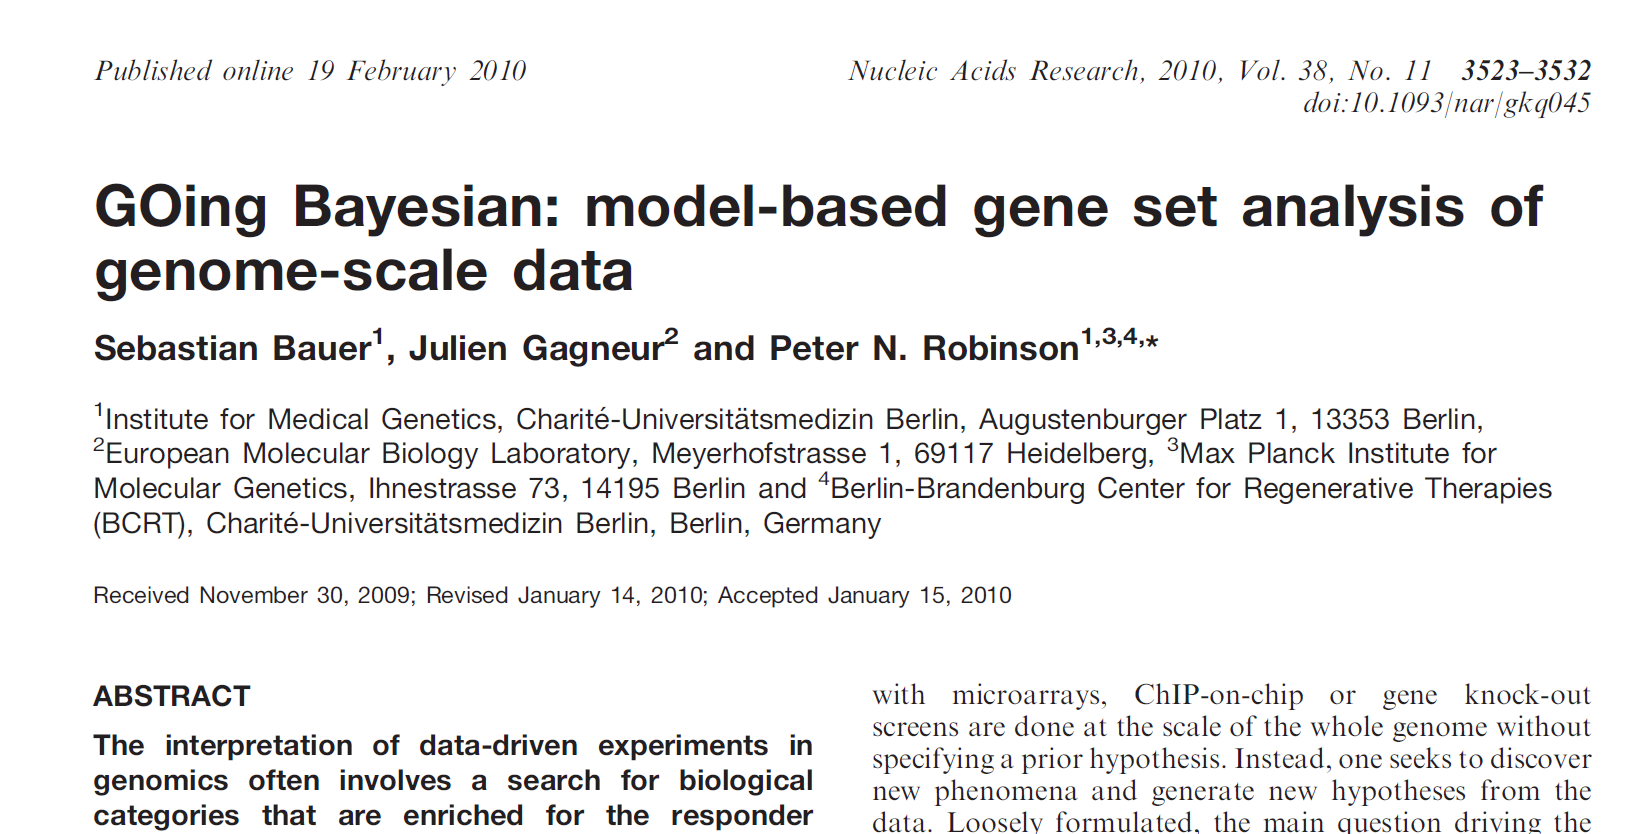
\includegraphics[width=0.6\textwidth]{./img/GOingBayesian-title.png}
\end{figure}


\end{frame}

%%%%%%%%%%%%%%%%%%%%%%%%%%%%%%%%%%%%%%%%%%%%%%%
%%%%%%%%%%%%%%%%%%%%%%%%%%%%%%%%%%%%%%%%%%%%%%%
\begin{frame}{Problems with the term for term approach}
 \begin{mybluebox}{What's the problem?}
A major difficulty of the
standard approach to GO overrepresentation analysis is that each term
is analyzed in isolation. 
 \end{mybluebox}
\begin{itemize}
 \item  Because of the statistical dependencies
between terms that are close to one another in the ontology graph, if
one term is called significant then commonly one or more related
terms are also called significant.
\end{itemize}


\end{frame}

%%%%%%%%%%%%%%%%%%%%%%%%%%%%%%%%%%%%%%%%%%%%%%%
%%%%%%%%%%%%%%%%%%%%%%%%%%%%%%%%%%%%%%%%%%%%%%%
\begin{frame}{Problems with the term for term approach}
 \begin{figure}
 \centering
 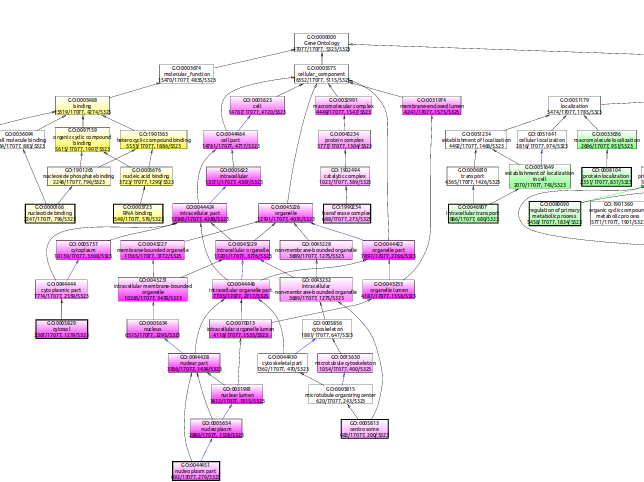
\includegraphics[width=0.6\textwidth]{./img/TfT-example.png}
\end{figure}

 \begin{itemize}
  \item Note how there seems to be a dependency between parent and child terms -- the distribution 
of significant terms is not uniform across all 44797 GO terms.
 \end{itemize}
\end{frame}

%%%%%%%%%%%%%%%%%%%%%%%%%%%%%%%%%%%%%%%%%%%%%%%
%%%%%%%%%%%%%%%%%%%%%%%%%%%%%%%%%%%%%%%%%%%%%%%
\begin{frame}{Model based gene-set analysis (MGSA)}
 \begin{mybluebox}{MGSA}
  MGSA is a completely different approach to GO
analysis that seeks to find the best combination of terms that
correspond to an experimental result.
 \end{mybluebox}

 \begin{itemize}
  \item The
problem reduces to an optimization problem, whereby the choice of
active GO terms, and optionally other parameters, are iteratively
varied in order to maximize a score or a probability.
\item   In contrast to
the algorithms in the last section, no statistical test (such as the
Fisher exact test or variants thereof) is performed for each term
\item Instead, there is a single score (or probability) that is to be
optimized for the entire set of GO terms.
 \end{itemize}

\end{frame}
%%%%%%%%%%%%%%%%%%%%%%%%%%%%%%%%%%%%%%%%%%%%%%%
%%%%%%%%%%%%%%%%%%%%%%%%%%%%%%%%%%%%%%%%%%%%%%%

\begin{frame}{GenGO}
 \begin{mybluebox}{Global optimization}
  A basic idea of MGSA is to fit a model on all the terms simultaneously, rather than testing each term in isolation. GenGO is a previous algorithm that attempts global optimization~\cite{Lu2008}
 \end{mybluebox}

\begin{columns}
\column{0.3\textwidth}
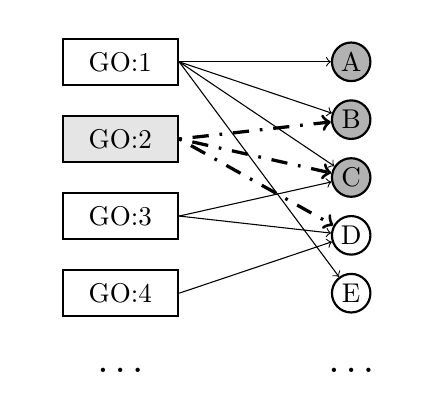
\includegraphics[width=1\textwidth]{./img/genGO.png}
\column{0.7\textwidth}
\begin{tiny}
\begin{itemize}
\item GO terms are modeled as active (gray) or
inactive (white) nodes that connect to the genes that are annotated to
them. 
\item The genes are either \texttt{ON} (gray) or \texttt{OFF}
(white). 
\item Intuitively speaking, the score in GenGO is maximized if a
set of GO terms is selected that are connected to as many of the
active genes as possible and as few of the inactive genes as possible.                               
\end{itemize}

\end{tiny}

\end{columns}



\end{frame}

%%%%%%%%%%%%%%%%%%%%%%%%%%%%%%%%%%%%%%%%%%%%%%%
%%%%%%%%%%%%%%%%%%%%%%%%%%%%%%%%%%%%%%%%%%%%%%%
\begin{frame}{GenGO (2)}
\begin{mybluebox}{Notation}
The GenGO algorithm defines several categories.
\end{mybluebox}

\begin{columns}

\column{0.75\textwidth}
\begin{scriptsize}
\begin{enumerate}
\item $\mathbf{A_g}$: \texttt{ON} gene node that is connected to at least one
  \texttt{active} GO term (e.g., genes B and C).
\item $\mathbf{A_n}$: \texttt{ON} gene node that is \textit{not} connected to any
  \texttt{active} GO term (e.g., gene A).
\item $\mathbf{I}$: \texttt{OFF} gene node (e.g., genes D and E).
\item $\mathbf{S_g}$: edge connecting  an \texttt{active} GO term with a node
  in $I$ (e.g., edge from \texttt{GO:2} to gene D).
\item $\mathbf{S_n}$: edge connecting  an \texttt{inactive} GO term with a node
  in $I$ (e.g., edge from \texttt{GO:4} to gene D).
\end{enumerate}
\end{scriptsize}
\column{0.25\textwidth}
 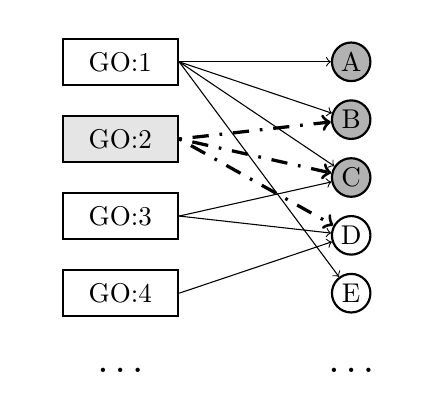
\includegraphics[width=1\textwidth]{./img/genGO.png}
\end{columns}

\end{frame}
%%%%%%%%%%%%%%%%%%%%%%%%%%%%%%%%%%%%%%%%%%%%%%%
%%%%%%%%%%%%%%%%%%%%%%%%%%%%%%%%%%%%%%%%%%%%%%%
\begin{frame}{GenGO (3)}
\begin{mybluebox}{GenGO model}
According to the model of genGO, GO terms can be ON or OFF, the ON terms activate genes and the OFF terms do not -- and then there is noise.
\end{mybluebox}

\begin{itemize}
 \item   an \texttt{active} GO term does not
activate all of the genes it annotated; rather, because of noise or
other errors, annotated genes are observed to be \texttt{OFF} with a
probability of $1-a$. 
\item Similarly, genes that are not annotated by any
\texttt{active} GO term are observed to be \texttt{ON} with a
probability of $b$. 
\item $a$ and $b$ are user-defined parameters or can be optimized by grid search (representative values are $a=0.9$ and $b=0.01$).
\end{itemize}

 
\end{frame}


%%%%%%%%%%%%%%%%%%%%%%%%%%%%%%%%%%%%%%%%%%%%%%%
%%%%%%%%%%%%%%%%%%%%%%%%%%%%%%%%%%%%%%%%%%%%%%%
\begin{frame}{GenGO (4)}
\begin{mybluebox}{GenGO model}
GenGO defines an objective function to be maximized,
\end{mybluebox}

\begin{itemize}
\item $C$ is the set of \texttt{active} GO terms in the current
iteration.
\end{itemize}

\begin{multline}
\mathcal{L}(C|p,q,G) = |A_g|\log a + |A_n|\log b  \\ + \; |S_g|\log (1-a)
+ |S_n| \log (1-b) - \alpha |C|
\label{eq:genGO}
\end{multline}
 
\end{frame}




%%%%%%%%%%%%%%%%%%%%%%%%%%%%%%%%%%%%%%%%%%%%%%%
%%%%%%%%%%%%%%%%%%%%%%%%%%%%%%%%%%%%%%%%%%%%%%%
\begin{frame}{GenGO (4)}
 The first four terms of Equation~(\ref{eq:genGO}) are equivalent to the
logarithm of the following equation
\begin{equation}
a^{|A_g|}b^{|A_n|}(1-a)^{|S_g|}(1-b)^{|S_n|}
\label{eq:genGO-no-log}
\end{equation}

\begin{columns}

\column{0.75\textwidth}
\begin{scriptsize}
Eq.~(\ref{eq:genGO-no-log}) is
maximized if $|A_g|>|S_g|$ (because  $a>1-a$) and if $|S_n|>|A_n|$
(because $1-b>b$). Thus, maximization of
Equation~(\ref{eq:genGO-no-log}) would tend to identify sets of
\texttt{active} GO terms
that more often than not annotate the \texttt{ON} genes
($|A_g|>|S_g|$). On the other hand, the \texttt{inactive} GO terms
would more often than not annotate \texttt{OFF} genes
($|S_n|>|A_n|$).
\end{scriptsize}
\column{0.25\textwidth}
 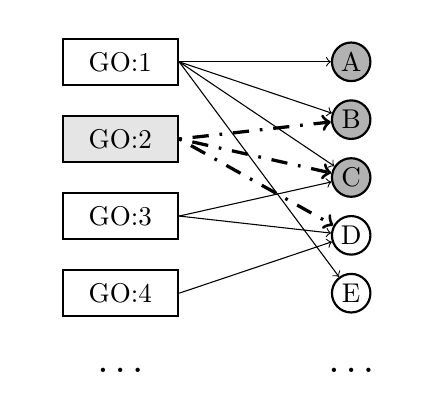
\includegraphics[width=1\textwidth]{./img/genGO.png}
\end{columns}


\end{frame}
%%%%%%%%%%%%%%%%%%%%%%%%%%%%%%%%%%%%%%%%%%%%%%%
%%%%%%%%%%%%%%%%%%%%%%%%%%%%%%%%%%%%%%%%%%%%%%%
\begin{frame}{GenGO (5)}

\begin{multline}
\mathcal{L}(C|p,q,G) = |A_g|\log a + |A_n|\log b  \\ + \; |S_g|\log (1-a)
+ |S_n| \log (1-b) \boxed{-\alpha |C|}
\label{eq:genGO}
\end{multline}
 
\begin{itemize}
\item The final term in Equation~(\ref{eq:genGO}), $- \alpha |C|$ reduces the
score linearly in the number of \texttt{active} GO terms.
\item The authors
of genGO state that a value of $\alpha=3$ tends to produce good
results. The genGO algorithm seeks to optimize the score for the
current set of \texttt{active} GO terms $C$. 
\end{itemize} 
 
\begin{mybluebox}{Magic numbers}
 Algorithms with ill defined heuristic parameters such as this may not perform well on datasets different to those they were originally tested on.
\end{mybluebox}
  
 
\end{frame}
%%%%%%%%%%%%%%%%%%%%%%%%%%%%%%%%%%%%%%%%%%%%%%%%%%%%%%%%%%%%%%%%%%%%%%%%%%%%%%%%%%%%%%%%%%%%%%%%%%%%
%%%%%%%%%%%%%%%%%%%%%%%%%%%%%%%%%%%%%%%%%%%%%%%%%%%%%%%%%%%%%%%%%%%%%%%%%%%%%%%%%%%%%%%%%%%%%%%%%%%%
\begin{frame}[fragile]{GenGO (6)}
  \begin{mybluebox}{Iterative algorithm}
  \begin{scriptsize}  
 In each iteration, the single-step change (removal or additional of a term)
 with the highest improvement of the score is chosen until no further
 improvement is possible.  \end{scriptsize}
 \end{mybluebox}
 \scalebox{.5}{   
\begin{algorithm}[H]
\KwData{study set $\mathcal{S}$, population set $\mathcal{P}$, 
     Gene Ontology $\mathcal{G}$, annotations $\mathcal{A}$}
 $C \leftarrow \emptyset$\;
\Repeat{No further improvement of score $\mathcal{L}(C)$}{
  \ForEach{$t \in \mathcal{G}$}{
      $t_L = \argmax_{t\in C} \mathcal{L} (C_i\backslash \left\{ t\right\} )$\;
      $t_M = \argmax_{t\in \mathcal{G}\setminus C} \mathcal{L} (C_i\cup \left\{ t\right\})$\;    
      \If{$\mathcal{L}(C_L) > \mathcal{L}(Ct_M)$} {
         $C = C\backslash \left\{ t\right\} )$\;
       } \ElseIf {$t_M > t_L$}  {
         $C = C\cup \left\{ t\right\} )$\;
       } 
    }
}
\Return{$C$}\;
\end{algorithm}
 }
 
 
\end{frame}

%%%%%%%%%%%%%%%%%%%%%%%%%%%%%%%%%%%%%%%%%%%%%%%%%%%%%%%%%%%%%%%%%%%%%%%%%%%%%%%%%%%%%%%%%%%%%%%%%%%%
%%%%%%%%%%%%%%%%%%%%%%%%%%%%%%%%%%%%%%%%%%%%%%%%%%%%%%%%%%%%%%%%%%%%%%%%%%%%%%%%%%%%%%%%%%%%%%%%%%%%
\begin{frame}[fragile]{GenGO (7)}
 \begin{mybluebox}{Improving upon GenGO}
 The idea behind
GenGO is  attractive because it represents a novel way
of avoiding the statistical dependency problems associated with the
overrepresentation methods described in the previous chapter.  
 \end{mybluebox}
\begin{itemize}
 \item However, the score and the optimization algorithm are heuristics without much statistical 
rigour
\item It seemed possible to improve upon this result using Bayesian methodologies
\end{itemize}

 
\end{frame}

%%%%%%%%%%%%%%%%%%%%%%%%%%%%%%%%%%%%%%%%%%%%%%%%%%%%%%%%%%%%%%%%%%%%%%%%%%%%%%%%%%%%%%%%%%%%%%%%%%%%
%%%%%%%%%%%%%%%%%%%%%%%%%%%%%%%%%%%%%%%%%%%%%%%%%%%%%%%%%%%%%%%%%%%%%%%%%%%%%%%%%%%%%%%%%%%%%%%%%%%%
\begin{frame}[fragile]{MGSA (1)}

\begin{itemize}
 \item Model-based gene set analysis (MGSA) is similar to
GenGO in that it seeks to identify an optimal combination of GO terms
to ``explain'' the results of microarray or other high-throughput
experiments. 
\item MGSA differs from genGO in that it embeds the GO terms and
the genes they annotate into a Bayesian network and uses probabilistic
methods to search for the optimal combination. 
\end{itemize}

\end{frame}
%%%%%%%%%%%%%%%%%%%%%%%%%%%%%%%%%%%%%%%%%%%%%%%%%%%%%%%%%%%%%%%%%%%%%%%%%%%%%%%%%%%%%%%%%%%%%%%%%%%%
%%%%%%%%%%%%%%%%%%%%%%%%%%%%%%%%%%%%%%%%%%%%%%%%%%%%%%%%%%%%%%%%%%%%%%%%%%%%%%%%%%%%%%%%%%%%%%%%%%%%
\begin{frame}[fragile]{MGSA (2)}
 \begin{itemize}
  \item 
Similar to genGO, MGSA assumes that the experiment attempts to detect genes that have a particular
\emph{state} (such as differential expression),
which can be \texttt{ON} or \texttt{OFF}. The true state of any gene is hidden. 
\item The
experiment and its associated analysis provide observations of the gene states
that are associated with unknown  false positive ($\alpha$) and  false negative rates
($\beta$), which we will assume to be identical and independent for all genes.

\item For instance, in the setting of a microarray experiment, the \texttt{ON} state
would correspond to differential expression, and the \texttt{OFF} state would
correspond to a lack of differential expression of a gene. Our model hence
assumes that differential expression is the consequence of the
annotation to some terms that are \texttt{active}.
 \end{itemize}

\end{frame}
%%%%%%%%%%%%%%%%%%%%%%%%%%%%%%%%%%%%%%%%%%%%%%%%%%%%%%%%%%%%%%%%%%%%%%%%%%%%%%%%%%%%%%%%%%%%%%%%%%%%
%%%%%%%%%%%%%%%%%%%%%%%%%%%%%%%%%%%%%%%%%%%%%%%%%%%%%%%%%%%%%%%%%%%%%%%%%%%%%%%%%%%%%%%%%%%%%%%%%%%%
\begin{frame}[fragile]{MGSA (3)}
 An additional parameter $p$ represents the prior probability of a term being
in the \texttt{active} state. The probability $p$ is typically low (less
than 0.5), which has the effect of introducing a penalization for
increasing the number of active terms. This favors results that
identify a relatively low number of \texttt{active} terms.
\end{frame}

%%%%%%%%%%%%%%%%%%%%%%%%%%%%%%%%%%%%%%%%%%%%%%%%%%%%%%%%%%%%%%%%%%%%%%%%%%%%%%%%%%%%%%%%%%%%%%%%%%%%
%%%%%%%%%%%%%%%%%%%%%%%%%%%%%%%%%%%%%%%%%%%%%%%%%%%%%%%%%%%%%%%%%%%%%%%%%%%%%%%%%%%%%%%%%%%%%%%%%%%%
\begin{frame}[fragile]{Structure of the MGSA Network}

  Gene
categories, or terms ($T_i$) that constitute the first layer can be either
\texttt{active} or \texttt{inactive}. Terms that are \texttt{active} activate the hidden state
($H_j$) of all genes annotated to them, with the other genes remaining \texttt{OFF}. The
observed states ($O_j$) of the genes are noisy observations of
their true hidden state. The parameters of the model (dashed nodes) are the
prior probability of each term to be \texttt{active}, $p$, the false positive rate, $\alpha$,
and the false negative rate, $\beta$.
\begin{figure}
 \centering
 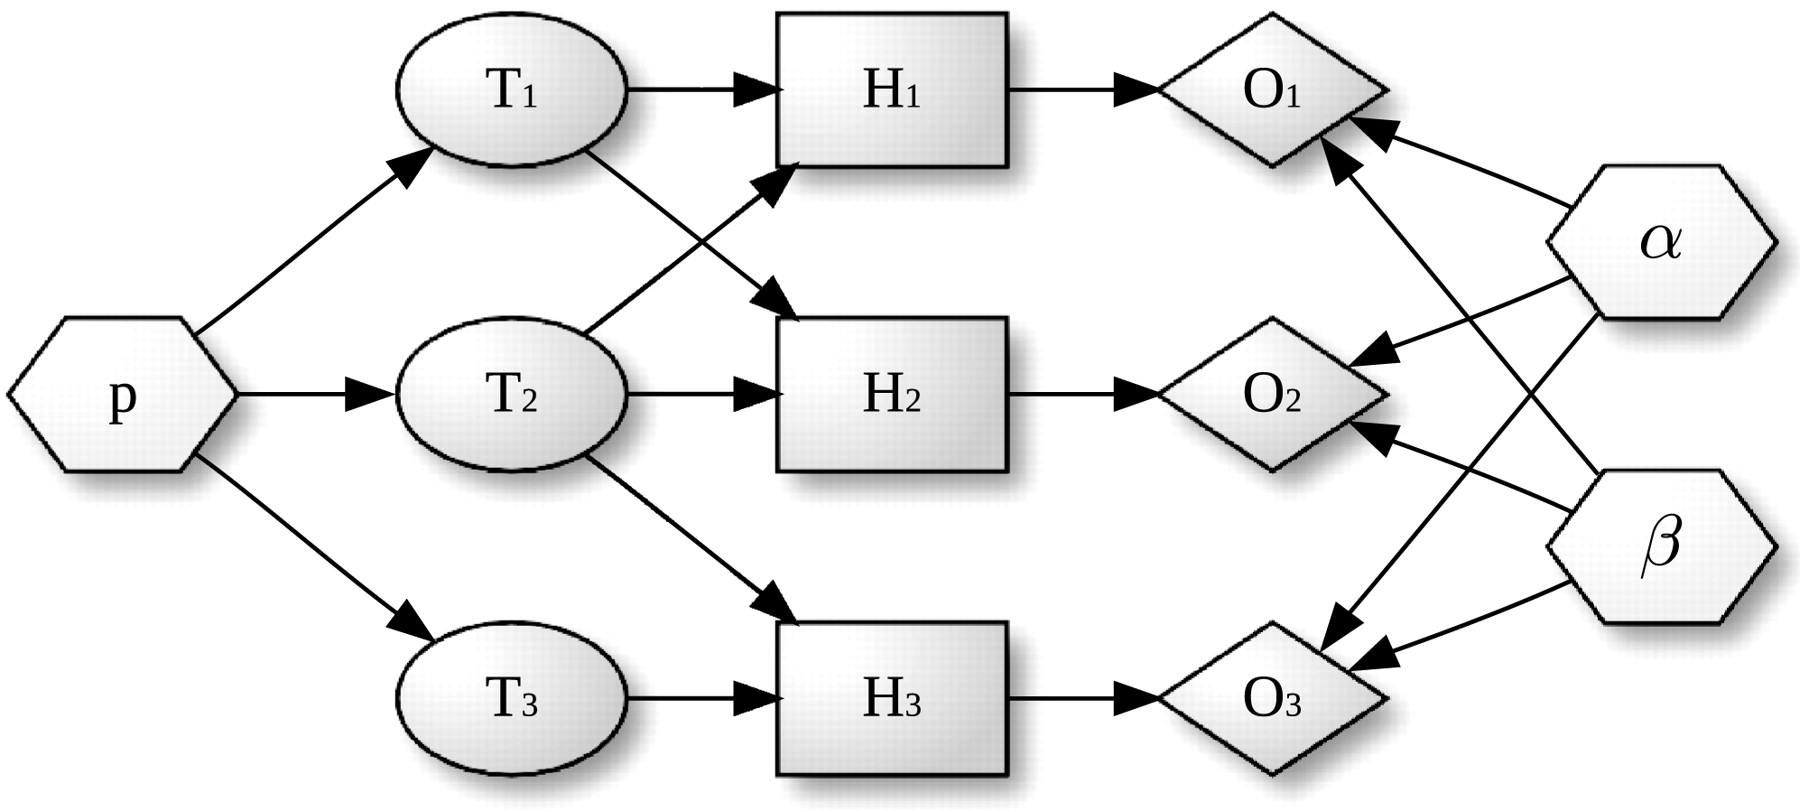
\includegraphics[width=0.6\textwidth]{./img/mgsa-F1.jpg}
\end{figure}

\end{frame}

%%%%%%%%%%%%%%%%%%%%%%%%%%%%%%%%%%%%%%%%%%%%%%%%%%%%%%%%%%%%%%%%%%%%%%%%%%%%%%%%%%%%%%%%%%%%%%%%%%%%
%%%%%%%%%%%%%%%%%%%%%%%%%%%%%%%%%%%%%%%%%%%%%%%%%%%%%%%%%%%%%%%%%%%%%%%%%%%%%%%%%%%%%%%%%%%%%%%%%%%%
\begin{frame}[fragile]{Structure of the MGSA Network}
 \begin{mybluebox}{Three layers: }
  More formally, the model can be described using a Bayesian network with three
layers that is augmented with a set of parameters.
 \end{mybluebox}
\begin{enumerate}
 \item A \emph{term layer} $T=\{T_1,\ldots,T_m\}$ that consists of Boolean nodes
 corresponding to $m$ terms of the ontology. There is a Boolean variable
 associated with each node that can have the state values \texttt{active} (1) or \texttt{inactive} 
(0). 
\end{enumerate}

 
 
\end{frame}

%%%%%%%%%%%%%%%%%%%%%%%%%%%%%%%%%%%%%%%%%%%%%%%%%%%%%%%%%%%%%%%%%%%%%%%%%%%%%%%%%%%%%%%%%%%%%%%%%%%%
%%%%%%%%%%%%%%%%%%%%%%%%%%%%%%%%%%%%%%%%%%%%%%%%%%%%%%%%%%%%%%%%%%%%%%%%%%%%%%%%%%%%%%%%%%%%%%%%%%%%
\begin{frame}[fragile]{Structure of the MGSA Network}

\begin{enumerate}
 \item \textcolor{gray}{A \emph{term layer}  }
 \item A \emph{hidden layer} $H=\{H_1,\ldots,H_n\}$ that contains Boolean nodes
 representing the $n$ annotated genes. There are edges
 from the terms to the genes they annotate.
 For instance, if gene $H_1$ is annotated to terms $T_1$ and $T_2$ then there is an edge between 
$T_1$ and $H_1$
 and another edge between $T_2$ and $H_1$. The state of the nodes reflects the
 true activation pattern of the genes. Each node can have the state
values \texttt{ON} (1), or \texttt{OFF} (0). 
\end{enumerate}
\end{frame}

%%%%%%%%%%%%%%%%%%%%%%%%%%%%%%%%%%%%%%%%%%%%%%%%%%%%%%%%%%%%%%%%%%%%%%%%%%%%%%%%%%%%%%%%%%%%%%%%%%%%
%%%%%%%%%%%%%%%%%%%%%%%%%%%%%%%%%%%%%%%%%%%%%%%%%%%%%%%%%%%%%%%%%%%%%%%%%%%%%%%%%%%%%%%%%%%%%%%%%%%%
\begin{frame}[fragile]{Structure of the MGSA Network}

\begin{enumerate}
 \item \textcolor{gray}{A \emph{term layer}  }
 \item \textcolor{gray}{A \emph{hidden layer}}
 \item An \emph{observed layer} $O=\{O_1,\ldots,O_n\}$ that contains Boolean
 nodes reflecting the state of all observed genes. The observed gene state nodes are
 directly connected to the corresponding hidden gene state nodes in a
 one-to-one fashion.
\end{enumerate}
\end{frame}
 
%%%%%%%%%%%%%%%%%%%%%%%%%%%%%%%%%%%%%%%%%%%%%%%%%%%%%%%%%%%%%%%%%%%%%%%%%%%%%%%%%%%%%%%%%%%%%%%%%%%%
%%%%%%%%%%%%%%%%%%%%%%%%%%%%%%%%%%%%%%%%%%%%%%%%%%%%%%%%%%%%%%%%%%%%%%%%%%%%%%%%%%%%%%%%%%%%%%%%%%%%
\begin{frame}[fragile]{Structure of the MGSA Network}

\begin{enumerate}
 \item \textcolor{gray}{A \emph{term layer}  }
 \item \textcolor{gray}{A \emph{hidden layer}}
 \item \textcolor{gray}{An \emph{observed layer} }
  \item A \emph{parameter set} that contains continuous nodes with values in
 $[0,1]$ corresponding to the parameters of the model $\alpha$, $\beta$ and
 $p$. These parameterize the distributions of the observed and the term layer
 as detailed below.
 
\end{enumerate}
\end{frame}
 
 
%%%%%%%%%%%%%%%%%%%%%%%%%%%%%%%%%%%%%%%%%%%%%%%%%%%%%%%%%%%%%%%%%%%%%%%%%%%%%%%%%%%%%%%%%%%%%%%%%%%%
%%%%%%%%%%%%%%%%%%%%%%%%%%%%%%%%%%%%%%%%%%%%%%%%%%%%%%%%%%%%%%%%%%%%%%%%%%%%%%%%%%%%%%%%%%%%%%%%%%%%
 \begin{frame}{The MGSA model}
  \begin{mybluebox}{MGSA--simplified}
   For didactic purposes, we will initially explain a simplified version
of MGSA in which the parameters $\alpha$, $\beta$ and $p$ are considered to
have known, fixed values.
  \end{mybluebox}



The state propagation of the nodes can be modeled using various \emph{local
probability distributions} (LPDs), denoted by $P$. The joint probability
distribution for this Bayesian network can be written as
\begin{multline}
  P(T,H,O) \; = \; P(T)P(H|T)P(O|H)\;  = P(T)\prod_{i=1}^n
  P(H_i|T) P(O_i|H_i).
\label{eqn:joint.general}
\end{multline}
 \end{frame}
%%%%%%%%%%%%%%%%%%%%%%%%%%%%%%%%%%%%%%%%%%%%%%%%%%%%%%%%%%%%%%%%%%%%%%%%%%%%%%%%%%%%%%%%%%%%%%%%%%%%
%%%%%%%%%%%%%%%%%%%%%%%%%%%%%%%%%%%%%%%%%%%%%%%%%%%%%%%%%%%%%%%%%%%%%%%%%%%%%%%%%%%%%%%%%%%%%%%%%%%%
 
\begin{frame}{T: The Term layer}

\begin{itemize}
 \item  The state of each term $T_j\in T$ is modeled according to a Bernoulli
distribution with hyperparameter $p$, i.e, $P(T_j=1)=p$. 
\item Denoting by
$\numberofterms{x}$ the number of terms that have state $x$ for a given $T$,
i.e., $\numberofterms{x}=|\{j|T_j=x\}|$. 
\end{itemize}

then
\begin{equation}
 P(T) = p^{\numberofterms{1}}(1-p)^{\numberofterms{0}}.
\label{eqn:prior}
\end{equation}
\begin{itemize}
 \item Thus, $p$ is the probability that a given term is ``on''.
\end{itemize}


\end{frame}
%%%%%%%%%%%%%%%%%%%%%%%%%%%%%%%%%%%%%%%%%%%%%%%%%%%%%%%%%%%%%%%%%%%%%%%%%%%%%%%%%%%%%%%%%%%%%%%%%%%%
%%%%%%%%%%%%%%%%%%%%%%%%%%%%%%%%%%%%%%%%%%%%%%%%%%%%%%%%%%%%%%%%%%%%%%%%%%%%%%%%%%%%%%%%%%%%%%%%%%%%

\begin{frame}{H: The hidden layer}
\begin{itemize}
\item  $T(H_i) \subseteq T$ is used to denote the set of
terms to which gene $H_i$ is annotated, i.e., the parents of $H_i$ in
the Bayesian network. 
\item For
the $T \rightarrow H$ links, any node $H_i \in H$ is \texttt{ON}
($H_i=1$) if at least one of its parents is \texttt{active}. Otherwise it
is \texttt{OFF}:
\end{itemize}




\begin{equation}
P(H_i=1|T) = \begin{cases}1, & \ifgenehasactiveterm \\ 0, &
\text{otherwise.} \end{cases}
%P(H_i|\emph{Pa}(H_i)) = \bigvee_{T\in\emph{Pa}(H_i)}T
\label{eqn:lpd.hidden.given.t}
\end{equation}
Note that this transition is deterministic.

\begin{itemize}
 \item The hidden nodes correspond to genes that are annotated by GO terms. If a GO term is ``ON'', 
then in the MGSA model any annotated gene is (truly) ``ON''.
\end{itemize}



\end{frame}
%%%%%%%%%%%%%%%%%%%%%%%%%%%%%%%%%%%%%%%%%%%%%%%%%%%%%%%%%%%%%%%%%%%%%%%%%%%%%%%%%%%%%%%%%%%%%%%%%%%%
%%%%%%%%%%%%%%%%%%%%%%%%%%%%%%%%%%%%%%%%%%%%%%%%%%%%%%%%%%%%%%%%%%%%%%%%%%%%%%%%%%%%%%%%%%%%%%%%%%%%


\begin{frame}{O: The observed layer}
 For the $H \rightarrow O$
connection, the following two Bernoulli distributions are used:

\begin{equation}
P(O_i=1|H_i=0) = \alpha
\label{eq:mgsa-bernoulli-alpha}
\end{equation}
and
\begin{equation}
P(O_i=0|H_i=1) = \beta.
\label{eq:mgsa-bernoulli-beta}
\end{equation}
\begin{itemize}
 \item The observed nodes correspond to the genes whose expression is observed by RNA-seq (etc.). According to our model, they may be ``OFF'', although the hidden node is 
``ON'' (false negative). 
\end{itemize}

 
\end{frame}
%%%%%%%%%%%%%%%%%%%%%%%%%%%%%%%%%%%%%%%%%%%%%%%%%%%%%%%%%%%%%%%%%%%%%%%%%%%%%%%%%%%%%%%%%%%%%%%%%%%%
%%%%%%%%%%%%%%%%%%%%%%%%%%%%%%%%%%%%%%%%%%%%%%%%%%%%%%%%%%%%%%%%%%%%%%%%%%%%%%%%%%%%%%%%%%%%%%%%%%%%


\begin{frame}{Fully specified MGSA Network}
 \begin{figure}
 \centering
 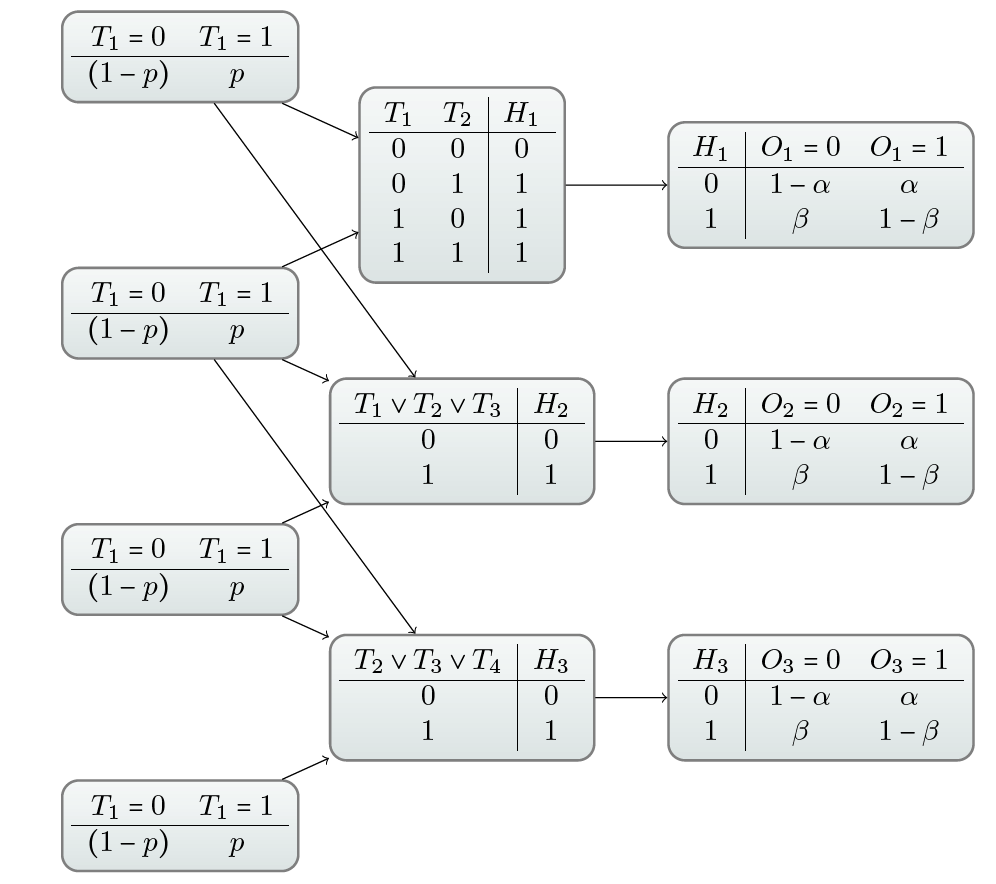
\includegraphics[width=0.6\textwidth]{./img/fullyspecifiedMGSA.png}
\end{figure}

 
\end{frame}

%%%%%%%%%%%%%%%%%%%%%%%%%%%%%%%%%%%%%%%%%%%%%%%%%%%%%%%%%%%%%%%%%%%%%%%%%%%%%%%%%%%%%%%%%%%%%%%%%%%%
%%%%%%%%%%%%%%%%%%%%%%%%%%%%%%%%%%%%%%%%%%%%%%%%%%%%%%%%%%%%%%%%%%%%%%%%%%%%%%%%%%%%%%%%%%%%%%%%%%%%


\begin{frame}{MGSA}

\begin{itemize}
 \item Denote by $\numberofgenes{x}{y} = |\left\{ i|O_{i}=x \wedge
  H_{i}=y\right\} |$ the number of genes having observed activation
$x$ and true activation $y$ according to the states of $T$. 
\item For
instance, $\numberofgenes{0}{1}$ corresponds to the number of genes
observed to be not differentially expressed but whose true activation
state is \textit{on}. 
\item Then, by considering the LPDs of nodes, one gets
the following product of Bernoulli distributions for $P(O|T)=
\prod_{i=1}^n P(H_i|T) P(O_i|H_i)$:
\end{itemize}

  


\begin{equation}
P(O|T) = \alpha^{\numberofgenes{1}{0}} (1 - \alpha)^{\numberofgenes{0}{0}}
(1-\beta)^{\numberofgenes{1}{1}} \beta^{\numberofgenes{0}{1}}.
\label{eq:alpha.beta.score}
\end{equation}
\end{frame}


 \begin{frame}{MGSA}
  \begin{equation}
P(O|T) = \alpha^{\numberofgenes{1}{0}} (1 - \alpha)^{\numberofgenes{0}{0}}
(1-\beta)^{\numberofgenes{1}{1}} \beta^{\numberofgenes{0}{1}}.
\label{eq:alpha.beta.score}
\end{equation}
\begin{itemize}
 \item Hence, Equation~(\ref{eq:alpha.beta.score}) calculates the product
of the probability of the observed states of the genes
given the hidden states of the terms. 
\item For instance, for $i=1$, we need
only consider hidden nodes whose parents include \texttt{active}
terms, because otherwise their probability is zero according to
Equation~(\ref{eqn:lpd.hidden.given.t}).
\item Using Equation~(\ref{eqn:prior})
with $p=\beta$, we obtain that $P(H_1|T) P(O_1|H_1)=1\times P(O_1|H_1) =
(1-\beta)^{\numberofgenes{1}{1}}
\beta^{\numberofgenes{0}{1}}$. 
\item Similar considerations for $i=0$ lead
to the final expression for Equation~(\ref{eq:alpha.beta.score}).
\end{itemize}

 \end{frame}
%%%%%%%%%%%%%%%%%%%%%%%%%%%%%%%%%%%%%%%%%%%%%%%%%%%%%%%%%%%%%%%%%%%%%%%%%%%%%%%%%%%%%%%%%%%%%%%%%%%%
%%%%%%%%%%%%%%%%%%%%%%%%%%%%%%%%%%%%%%%%%%%%%%%%%%%%%%%%%%%%%%%%%%%%%%%%%%%%%%%%%%%%%%%%%%%%%%%%%%%%


\begin{frame}{MAP: Maximum a postgeriori}
 \begin{mybluebox}{MAP}
   In Bayesian statistics, maximum a posteriori (MAP) estimation is often
used to generate an estimate of the maximum value of a probability
distribution. 
 \end{mybluebox}

That is, if $x$ is used to refer to the data ($x$ can be
an arbitrary expression), and $\theta$ is used to refer to the
parameters of a model, then Bayes' law states that:

\begin{equation}
P(\theta | x) = \dfrac{P(x|\theta )P(\theta )}{P(x)}
\label{eq:bayes-law-for-map}
\end{equation}
 
\end{frame}
%%%%%%%%%%%%%%%%%%%%%%%%%%%%%%%%%%%%%%%%%%%%%%%%%%%%%%%%%%%%%%%%%%%%%%%%%%%%%%%%%%%%%%%%%%%%%%%%%%%%
%%%%%%%%%%%%%%%%%%%%%%%%%%%%%%%%%%%%%%%%%%%%%%%%%%%%%%%%%%%%%%%%%%%%%%%%%%%%%%%%%%%%%%%%%%%%%%%%%%%%


\begin{frame}{MAP: Maximum a posteriori}
 \begin{itemize}
  \item The term $P(\theta | x)$ is referred to as the posterior probability,
and specifies the probability of the parameters $\theta$ given the
observed data $x$. 
\item The denominator on the right-hand side can be
regarded as a normalizing constant that does not depend on $\theta$,
and so it can be disregarded for the maximization of $\theta$. 
\item The MAP
estimate of $\theta$ is defined as:
 \end{itemize}


\begin{equation}
\argmax_{\theta} P(\theta | x) = \argmax_{\theta} P(x|\theta )(P(\theta )
\label{eq:map}
\end{equation}
 
 
\end{frame}
%%%%%%%%%%%%%%%%%%%%%%%%%%%%%%%%%%%%%%%%%%%%%%%%%%%%%%%%%%%%%%%%%%%%%%%%%%%%%%%%%%%%%%%%%%%%%%%%%%%%
%%%%%%%%%%%%%%%%%%%%%%%%%%%%%%%%%%%%%%%%%%%%%%%%%%%%%%%%%%%%%%%%%%%%%%%%%%%%%%%%%%%%%%%%%%%%%%%%%%%%


\begin{frame}{MAP: Maximum a posteriori}
 \begin{itemize}
  \item  In the case of MGSA, the parameters comprised by $\theta$ would
include the set of \texttt{active} terms as well as values for
$\alpha,\beta$, and $p$. 

\item Although MAP estimation procedures are often relatively simple to
implement, they tend to have the disadvantage that they ``get stuck'' in
local maxima  without being
able to offer a guarantee of finding the global maximum.
 \end{itemize}

 \begin{figure}
 \centering
 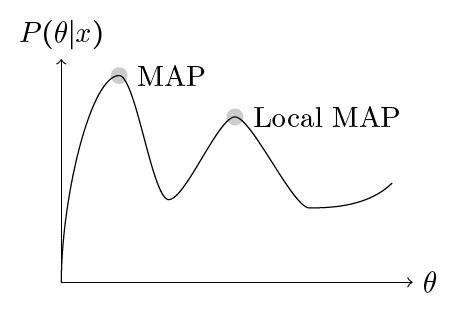
\includegraphics[width=0.5\textwidth]{./img/MAP.png}
\end{figure}

 
\end{frame}
%%%%%%%%%%%%%%%%%%%%%%%%%%%%%%%%%%%%%%%%%%%%%%%%%%%%%%%%%%%%%%%%%%%%%%%%%%%%%%%%%%%%%%%%%%%%%%%%%%%%
%%%%%%%%%%%%%%%%%%%%%%%%%%%%%%%%%%%%%%%%%%%%%%%%%%%%%%%%%%%%%%%%%%%%%%%%%%%%%%%%%%%%%%%%%%%%%%%%%%%%


\begin{frame}{MAP: Shortcomings?}
 
 \begin{itemize}
  \item  In
complicated networks such as that of MGSA, it is \textbf{rare to have a single
solution} that is substantially better than all alternative
solutions. 
\item Rather, the posterior probability is usually spread over a
number of alternative network configurations. This implies that the
posterior probability is not adequately represented by a single
configuration $\theta^{MAP}$
\item It is more appropriate to
sample networks from the posterior probability, leading to a
\textbf{collection of networks with high posterior probability}, each of
which offers a good explanation of the data. 
 \end{itemize}
\begin{mybluebox}{MCMC}
These considerations motivate the
use of the MCMC algorithm to sample from the posterior distribution.
\end{mybluebox}

 
 
\end{frame}
%%%%%%%%%%%%%%%%%%%%%%%%%%%%%%%%%%%%%%%%%%%%%%%%%%%%%%%%%%%%%%%%%%%%%%%%%%%%%%%%%%%%%%%%%%%%%%%%%%%%
%%%%%%%%%%%%%%%%%%%%%%%%%%%%%%%%%%%%%%%%%%%%%%%%%%%%%%%%%%%%%%%%%%%%%%%%%%%%%%%%%%%%%%%%%%%%%%%%%%%%


\begin{frame}{MAP: Shortcomings?}
 
 \begin{figure}
 \centering
 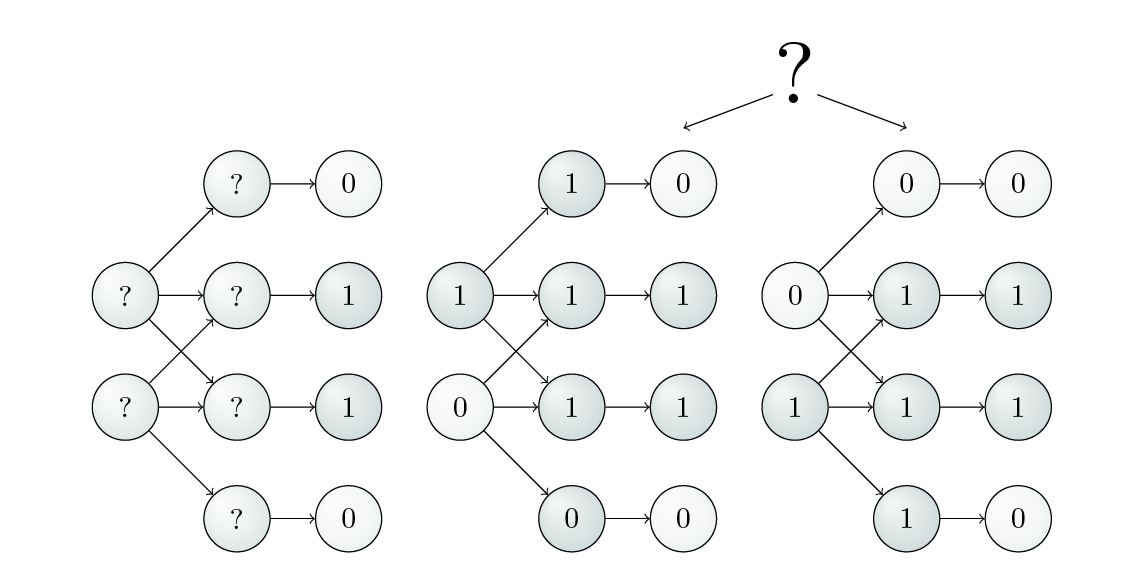
\includegraphics[width=0.8\textwidth]{./img/MGSA-twonetworks.png}
 % MGSA-twonetworks.png: 0x0 pixel, 300dpi, 0.00x0.00 cm, bb=
\end{figure}
\begin{tiny}\begin{itemize}
 \item  the optimization problem addressed by
  genGO and MGSA is known to be NP-complete. 
  \item  We observe that
  gene 2 and 3 are in the \texttt{ON} state (e.g., differentially
  expressed).
  \item  If $T_1$ were the only \texttt{active} term, then the observation
  could be explained by risking an error of one false-negative. The
  same can be noticed if $T_2$ is the only \texttt{active} term.
  \item thus there is no
  single optimum solution. A single MAP solution does not account for
  this.
\end{itemize}             
\end{tiny}

\end{frame}



%%%%%%%%%%%%%%%%%%%%%%%%%%%%%%%%%%%%%%%%%%%%%%%%%%%%%%%%%%%%%%%%%%%%%%%%%%%%%%%%%%%%%%%%%%%%%%%%%%%%
%%%%%%%%%%%%%%%%%%%%%%%%%%%%%%%%%%%%%%%%%%%%%%%%%%%%%%%%%%%%%%%%%%%%%%%%%%%%%%%%%%%%%%%%%%%%%%%%%%%%


\begin{frame}{Monte Carlo Markov Chain (MCMC) Algorithm}
 \begin{itemize}
  \item A different approach is to calculate the marginal probabilities for
each term being in the \texttt{active} state. 
\item In general, if a joint
probability is defined over two random variables $X$ and $Y$ as
$P(X,Y)=P(X|Y)P(Y)$, then the marginal
probability for $X=x'$ is calculated by summing or integrating over all
possible values of $Y$:
\begin{equation}
 P(X=x')=\sum_{i} P(X=x',Y=y_i)
\end{equation}


  or
  \begin{equation}
   P(X=x')=\int_Y P(X=x',Y) \mathrm{d}Y
  \end{equation}


 \end{itemize}

 

\end{frame}

%%%%%%%%%%%%%%%%%%%%%%%%%%%%%%%%%%%%%%%%%%%%%%%%%%%%%%%%%%%%%%%%%%%%%%%%%%%%%%%%%%%%%%%%%%%%%%%%%%%%
%%%%%%%%%%%%%%%%%%%%%%%%%%%%%%%%%%%%%%%%%%%%%%%%%%%%%%%%%%%%%%%%%%%%%%%%%%%%%%%%%%%%%%%%%%%%%%%%%%%%


\begin{frame}{MCMC}
 \begin{itemize}
  \item It is often difficult or
impossible to derive marginal probabilities for complicated
probability distributions because there are simply too many possible
configurations of the variables to be able to calculate each one. 
\item Estimation algorithms sample from the distribution of the posterior probability and take the
proportion of samples in which $X$ takes on some specific value
$x'$ as an estimate of the posterior probability of $x'$  
 \end{itemize}
\begin{mybluebox}{MCMC}
 One of the best known and most effective algorithms for this purpose
is the Metropolis-Hasting algorithm, which is a Markov chain Monte
Carlo (MCMC) method. The
MCMC algorithm performs a random walk over the term and parameter
configurations, which asymptotically provides a random sampler
according to the target distribution $P(T|O)$.
\end{mybluebox}
\end{frame}
%%%%%%%%%%%%%%%%%%%%%%%%%%%%%%%%%%%%%%%%%%%%%%%%%%%%%%%%%%%%%%%%%%%%%%%%%%%%%%%%%%%%%%%%%%%%%%%%%%%%
%%%%%%%%%%%%%%%%%%%%%%%%%%%%%%%%%%%%%%%%%%%%%%%%%%%%%%%%%%%%%%%%%%%%%%%%%%%%%%%%%%%%%%%%%%%%%%%%%%%%
\begin{frame}{MCMC}
 Given the current configuration of the terms denoted by $T^t$, the algorithm
proposes a neighbor state $T^p$ in accordance to a proposal density function
$Q_T(\cdot|T^t)$. A value $r$ is sampled uniformly from the range (0,1). Then,
if
\begin{equation}
 r < P_{\text{accept}}(T^t,T^p) = 
 \frac{P(T^{p}|O)Q_T(T^{t}|T^{p})}{P(T^{t}|O)Q_T(T^{p}|T^t)}
 \label{eqn:acceptance}
\end{equation}
the proposal is accepted, then we choose the proposed state, i.e., $T^{t+1} = T^p$, otherwise it is rejected,
i.e., $T^{t+1} = T^t$.
\end{frame}
%%%%%%%%%%%%%%%%%%%%%%%%%%%%%%%%%%%%%%%%%%%%%%%%%%%%%%%%%%%%%%%%%%%%%%%%%%%%%%%%%%%%%%%%%%%%%%%%%%%%
%%%%%%%%%%%%%%%%%%%%%%%%%%%%%%%%%%%%%%%%%%%%%%%%%%%%%%%%%%%%%%%%%%%%%%%%%%%%%%%%%%%%%%%%%%%%%%%%%%%%
\begin{frame}{MCMC}
 
 Using Bayes' law, we have
\begin{equation}
 P(T^{p}|O) = \dfrac{P(O|T^{p})P(T^{p})}{P(O)}
 \label{eqn:cond.prob}
\end{equation}
and similarly for $T^{t}$. Substituting these expressions for $P(T^{p}|O)$ and
$P(T^{t}|O)$ cancels out the normalization constant $P(O)$. The acceptance
probability is then:
\begin{equation}
 P_{\text{accept}}(T^t,T^p) = 
 \frac{P(O|T^{p})P(T^{p})Q_T(T^{t}|T^{p})}{P(O|T^{t})P(T^{t})Q_T(T^{p}|T^t)}.
\label{eqn:accept.prop.2}
\end{equation}
 \begin{itemize}
  \item We have $P(O|T)$ and $P(T)$ from the statement of the MGSA network
 \end{itemize}

\end{frame}
%%%%%%%%%%%%%%%%%%%%%%%%%%%%%%%%%%%%%%%%%%%%%%%%%%%%%%%%%%%%%%%%%%%%%%%%%%%%%%%%%%%%%%%%%%%%%%%%%%%%
%%%%%%%%%%%%%%%%%%%%%%%%%%%%%%%%%%%%%%%%%%%%%%%%%%%%%%%%%%%%%%%%%%%%%%%%%%%%%%%%%%%%%%%%%%%%%%%%%%%%
\begin{frame}{MCMC}
 Equation (\ref{eqn:accept.prop.2}) is used iteratively to define a
random walk through the space of configurations.  A \emph{burn-in
  period} consisting of a certain number of iterations is used to
initialize the MCMC chain (in our implementation of the MGSA algorithm
in the Ontologizer, the default is 20,000
iterations). Following this, $l$ further iterations (by default,
$10^6$) are performed.  Let $C(T_i)$ be the number of samples in which
term $T_i$ was \texttt{active}. Then

\begin{equation}
P(T_i|O)\approx \frac{C(T_i)}{l}.
\label{eqn:mgsa-marginal}
\end{equation}
 
 
\end{frame}
%%%%%%%%%%%%%%%%%%%%%%%%%%%%%%%%%%%%%%%%%%%%%%%%%%%%%%%%%%%%%%%%%%%%%%%%%%%%%%%%%%%%%%%%%%%%%%%%%%%%
%%%%%%%%%%%%%%%%%%%%%%%%%%%%%%%%%%%%%%%%%%%%%%%%%%%%%%%%%%%%%%%%%%%%%%%%%%%%%%%%%%%%%%%%%%%%%%%%%%%%
\begin{frame}{MCMC}
\begin{mybluebox}{proposal density function}
 In order to finish the description of the algorithm, one needs to define
classes of operations of which a proposal is chosen, that is, we need to
specify $Q_T(T^p|T^t)$.
\end{mybluebox}


  Denote by $T^p \leftrightarrow_T T^t$ the binary
relation that  states  that $T^p$   be constructed from $T^t$ by either
\begin{itemize}
  \item toggling the \texttt{active}/\texttt{inactive} state of a single term, or by
  \item exchanging the state of a pair of terms that contains a single
    \texttt{active} term and a single \texttt{inactive} term.
\end{itemize}
\end{frame}
%%%%%%%%%%%%%%%%%%%%%%%%%%%%%%%%%%%%%%%%%%%%%%%%%%%%%%%%%%%%%%%%%%%%%%%%%%%%%%%%%%%%%%%%%%%%%%%%%%%%
%%%%%%%%%%%%%%%%%%%%%%%%%%%%%%%%%%%%%%%%%%%%%%%%%%%%%%%%%%%%%%%%%%%%%%%%%%%%%%%%%%%%%%%%%%%%%%%%%%%%
\begin{frame}{MCMC}
 Denote by $N(T)$ the \emph{neighborhood} of a given configuration for
$T$, that is, the number of different operations that can be applied
once to $T$ in order to get a new configuration. At first, there are
$m$ terms in total, each of which can be toggled. In addition, there
are $\numberofterms{0}\numberofterms{1}$ possibilities to combine
terms that are \texttt{active} with terms that are \texttt{inactive}.
Thus, there are a total of $N(T)=m+\numberofterms{0}\numberofterms{1}$
valid state transitions. We would like to sample the valid proposals
with equal probability; therefore, the proposal distribution $Q_T$ is
determined by
\begin{equation}
 Q_T(T^p|T^t)=\begin{cases}
                  \frac{1}{N(T^t)}, & \text{if } T^p \leftrightarrow_T
                  T^t\\ 0, & \text{otherwise.}
               \end{cases},
\end{equation}
which we can use to rewrite Equation~(\ref{eqn:accept.prop.2}) to:

\newcommand{\acceptratio}{\frac{P(O|T^{p})P(T^{p})N(T^t)}{P(O|T^{t})P(T^{t})N(T^p)}}
\begin{equation*}
 P_{\text{accept}}(T^t,T^p) = 
 \acceptratio.
\label{eqn:accept.prop.3}
\end{equation*}
\end{frame}

%%%%%%%%%%%%%%%%%%%%%%%%%%%%%%%%%%%%%%%%%%%%%%%%%%%%%%%%%%%%%%%%%%%%%%%%%%%%%%%%%%%%%%%%%%%%%%%%%%%%
%%%%%%%%%%%%%%%%%%%%%%%%%%%%%%%%%%%%%%%%%%%%%%%%%%%%%%%%%%%%%%%%%%%%%%%%%%%%%%%%%%%%%%%%%%%%%%%%%%%%

\begin{frame}{MCMC State transitions for MGSA}
 \begin{figure}
 \centering
 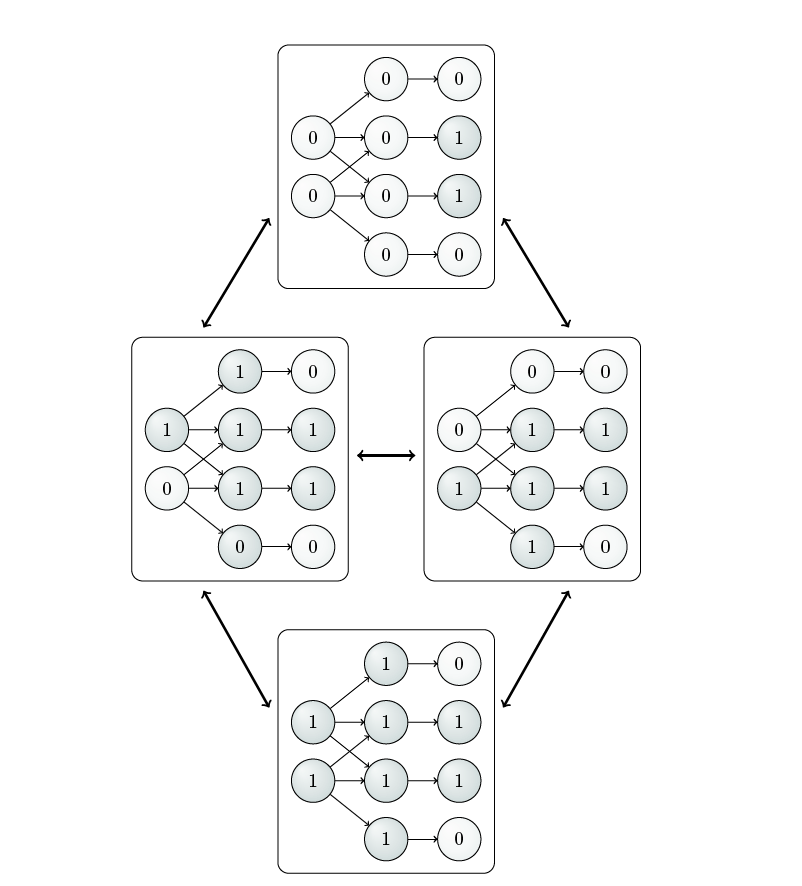
\includegraphics[width=0.5\textwidth]{./img/MGSAtransitions.png}
\end{figure}

\end{frame}
%%%%%%%%%%%%%%%%%%%%%%%%%%%%%%%%%%%%%%%%%%%%%%%%%%%%%%%%%%%%%%%%%%%%%%%%%%%%%%%%%%%%%%%%%%%%%%%%%%%%
%%%%%%%%%%%%%%%%%%%%%%%%%%%%%%%%%%%%%%%%%%%%%%%%%%%%%%%%%%%%%%%%%%%%%%%%%%%%%%%%%%%%%%%%%%%%%%%%%%%%
\newcommand{\acceptratio}{\frac{P(O|T^{p})P(T^{p})N(T^t)}{P(O|T^{t})P(T^{t})N(T^p)}}
\begin{frame}[fragile]{MGSA}
 \scalebox{.7}{   
\begin{algorithm}[H]
\KwData{$O$, $l$ (number of steps)}
\KwResult{$P(T_1=1|O),\ldots,P(T_m=1|O))$}
 $T^t \leftarrow \underbrace{(0,\ldots,0)}_{m\textrm{ times}}$;
   \For{$t \leftarrow 1$ \KwTo $l$}{
    $T^p \sim Q_T(\cdot|T^t)$, i.e., choose a neighbor candidate by either
    \begin{itemize}
        \item toggling a term
        \item exchanging an active term with an inactive one
      \end{itemize} 
       $a \leftarrow \acceptratio$;
        $r \sim U(0,1)$; \\
	\If{$r < a$}{
		$T^t \leftarrow T^p$
	}
   }
\Return{$\left(\frac{C(T_1)}l,\ldots,\frac{C(T_m)}l\right)$}
\end{algorithm}
 }


A Metropolis-Hasting algorithm to estimate $P(T_i=1|O)$.

\begin{tiny}For simplicity, the
burn-in period was omitted from the pseudocode.\end{tiny}
\end{frame}


\begin{frame}{MGSA: Evaluation}

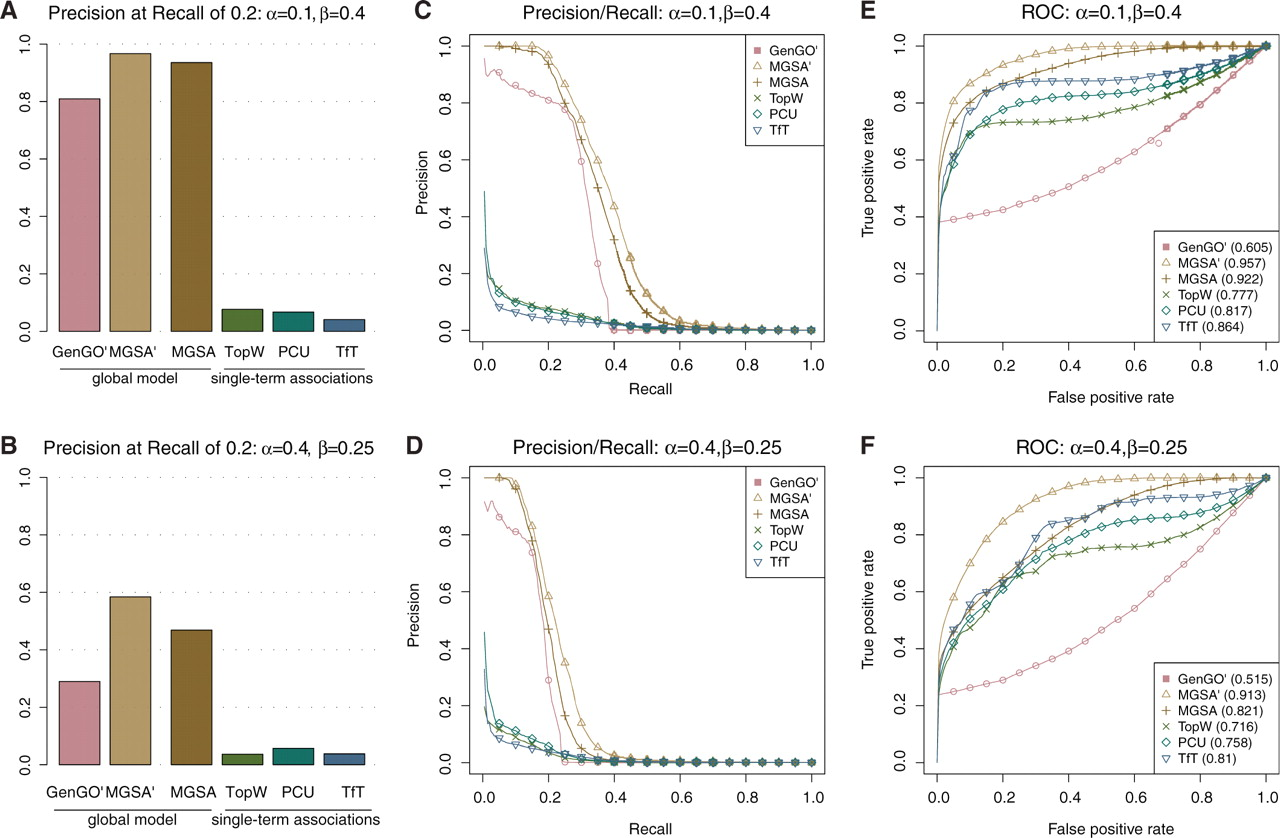
\includegraphics[width=1\textwidth]{img/mgsa-F2.jpg} 
\end{frame}

\begin{frame}{MGSA: Example}

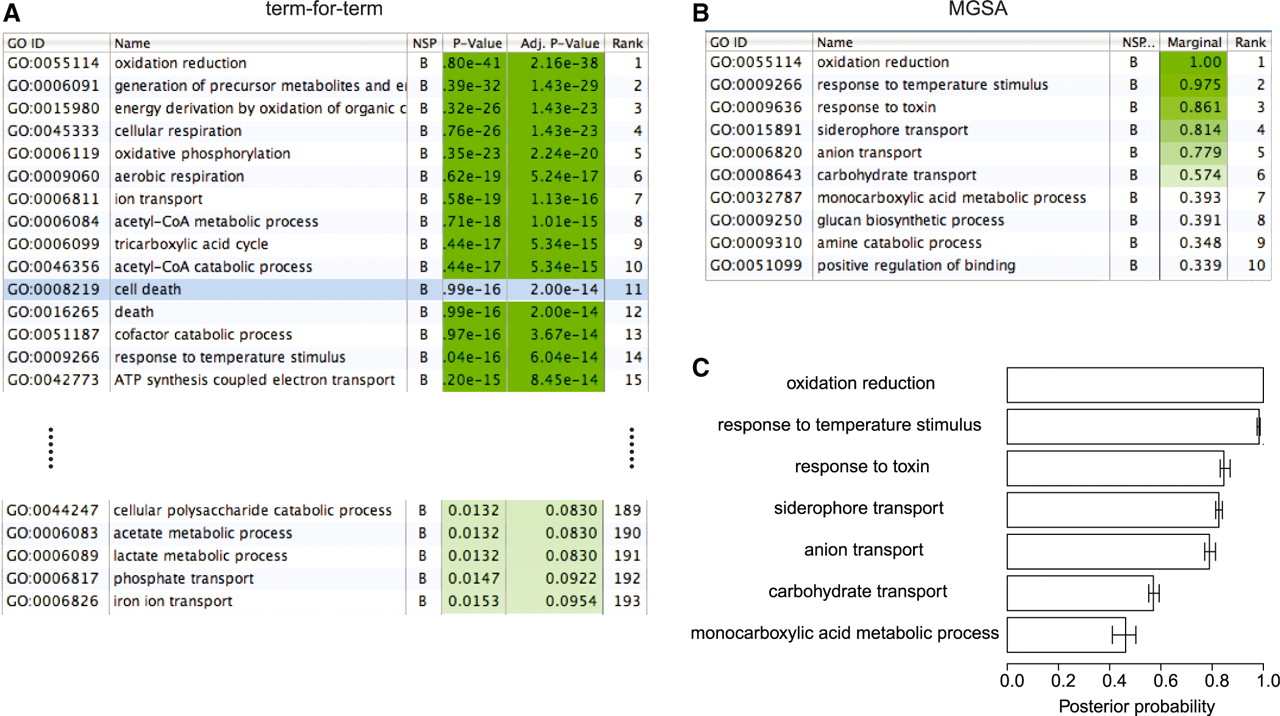
\includegraphics[width=1\textwidth]{img/mgsa-F3.jpg} 
\end{frame}

\appendix

\begin{frame}{References}
	\nocite{*} % Display all references regardless of if they were cited
	\bibliography{semalgs.bib}
	\bibliographystyle{plain}
\end{frame}
%------------------------------------------------
\end{document}
\begin{frame}{Blocks}
	These blocks are part of 1 slide, to be displayed consecutively.
	\begin{block}{Block}
		Text.
	\end{block}
	\pause % Automatically creates a new "page" split between the above and above + below
	\begin{alertblock}{Alert block}
		Alert \alert{text}.
	\end{alertblock}
	\pause % Automatically creates a new "page" split between the above and above + below
	\begin{exampleblock}{Example block}
		Example \textcolor{example}{text}.
	\end{exampleblock}
\end{frame}


%----------------------------------------------------------------------------------------
%	 CLOSING/SUPPLEMENTARY SLIDES
%----------------------------------------------------------------------------------------



%------------------------------------------------

\begin{frame}{Backup Slide}
	This is a backup slide, useful to include additional materials to answer questions from the audience.
	\vfill
	The package \texttt{appendixnumberbeamer} is used to refrain from numbering appendix slides.
\end{frame}

%----------------------------------------------------------------------------------------

\end{document}
